\documentclass[a4paper,12pt,times,numbered,print,index]{template/PhDThesisPSnPDF}

% TODO, remove before submission
\newcommand\todo[1]{\textcolor{red}{TODO: #1}}

\usepackage{subfig}

% define metadata like author, title
% ************************ Thesis Information & Meta-data **********************
%% The title of the thesis
\title{Articulated Tracking for Humanoid Manipulation}
%\texorpdfstring is used for PDF metadata. Usage:
%\texorpdfstring{LaTeX_Version}{PDF Version (non-latex)} eg.,
%\texorpdfstring{$sigma$}{sigma}

%% Subtitle (Optional)
%\subtitle{Using the CUED template}

%% The full name of the author
\author{Christian Rauch}

%% Department (eg. Department of Engineering, Maths, Physics)
\dept{School of Informatics}

%% University and Crest
\university{University of Edinburgh}
% Crest minimum should be 30mm.
\crest{
\includegraphics[width=0.5\textwidth]{logo/UoE_Logo.eps}}
%% Use this crest, if you are using the college crest
%% Crest long miminum should be 65mm
%\crest{\includegraphics[width=0.45\textwidth]{University_Crest_Long}}

%% College shield [optional] 
% Crest minimum should be 30mm.
%\collegeshield{\includegraphics[width=0.2\textwidth]{CollegeShields/Kings}}


%% Supervisor (optional)
%% for multiple supervisors, append each supervisor with the \newline command
%\supervisor{\textbf{Prof. A.B. Supervisor\newline
%Prof. C.D. Supervisor\newline
%Prof. E.F. Supervisor\newline
%Prof. G.H. Supervisor}}

%% Supervisor Role (optional) - Supervisor (default) or advisor
% \supervisorrole{\textbf{Supervisors: }}
%% if no title is desired:
% \supervisorrole{}

%% Advisor (optional)
%% for multiple advisors, append each advisor with the \newline command
%\advisor{Advisor 1\newline
%Advisors 2\newline
%Advisor 3\newline
%Advisor 4}
     
%% Advisor Role (optional) - Advisor (default) or leave empty
% \advisorrole{Advisors: }
%% if no title is required
% \advisorrole{}


%% You can redefine the submission text:
% Default as per the University guidelines:
% ``This dissertation is submitted for the degree of''
%\renewcommand{\submissiontext}{change the default text here if needed}

%% Full title of the Degree
\degreetitle{Master of Science by Research}

%% College affiliation (optional)
%\college{King's College}

%% Submission date
% Default is set as {\monthname[\the\month]\space\the\year}
\degreedate{August 2016} 

%% Meta information
%\subject{LaTeX} \keywords{{LaTeX} {PhD Thesis} {Engineering} {University of
%Cambridge}}


% main document
\begin{document}

\frontmatter
\maketitle
\tableofcontents
\listoffigures
%\listoftables

\mainmatter

% chapters
\chapter{Introduction}

\section{Motivation}

Amongst all robot types, humanoid robots are one of the most versatile robots when it comes to acting in a world with man-made structures and tools. As such, they are a huge area of research involving multiple disciplines. Of special research interest is humanoid manipulation using manipulators that resemble human hands. Manipulators with several degree of freedom enable robots to reuse man-made tools for solving different kind of problems as opposed to be restricted to task-specific manipulators. Some of the tasks defined for the DARPA robotics challenge 2015 (DRC) \cite{DRC2013} intended to advance robotic manipulation into this direction by setting a robot in a rescue scenario that involves the interaction with door handles (Door task), turning valves (Valve task), connecting a hose to a wye (Hose task) and using a drill to cut a hole in a wall (Wall task). Since the DRC rules stated that the robot needed to carry all of its manipulators during each trial, teams were force to use versatile manipulators.

The advantage of having such a generic manipulator comes with the cost of more complex control. Humanoid manipulation does not only involve the grasping of a tool but also the continuous control of this tool for the duration of the task. Since grasped tools are only indirectly connected to the robot's kinematic chain, additional perceptual information is needed to estimate and track the actual state of the manipulated object.


\section{Problem Definition and Research Aim}

Humanoid manipulation is a challenging task because of two main reasons: inaccurate forward kinematics and changing environment.
Inaccurate forward kinematics is mostly caused by improper calibrated joint encoders and linkage elasticity. Both issues can only be resolved to some extent by e.g. modelling joint position offsets \cite{Fallon2015} and stiffness coefficients \cite{Johnson2015}. The effect of inaccurate forward kinematics is visualised in \cref{fig:calibration_issue}. Even small deviations in the reported joint positions propagate through the kinematic chain towards the manipulator and result in an offset that makes open-loop grasping infeasible.
By interacting with objects such as a valve, the robot needs to compensate the applied force by a whole body motion which likely changes the pose of the manipulated object in the camera frame.

\begin{figure}
\captionsetup{width=0.6\textwidth}
\centering
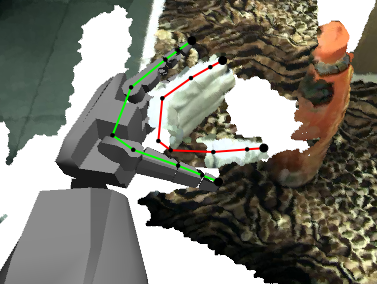
\includegraphics[width=0.5\textwidth]{images/valkyrie/joint_calibration_issue.png}
\caption[Joint calibration issue]{Joint calibration issue resulting in offset of reported pose (solid gray mesh, green marker) from perceived hand pose (coloured point cloud, red marker).}
\label{fig:calibration_issue}
\end{figure}

Both issues are in contrast with open-loop industrial robot applications such as moving parts in an assembly line, where stiff actuators manipulate objects at defined poses. Using visual feedback to estimate the configuration of the manipulator and the pose of the manipulated object could be the key step to enable closed-loop manipulation.
In return, visual tracking of highly articulated manipulators and objects causes interesting research questions itself again.

\paragraph{Manipulator tracking}
The main problem of tracking highly articulated manipulators with several degree of freedom is the large variety of their appearance. Using classical object detection methods on this problem would require an enormous amount of training data containing different configurations at different lighting conditions. In addition, classification results must be provided at real-time. On one side, the problem can be simplified in the context where a robot is observing its own manipulator by using a robot model representation and its joint encoder values. On the other side, the before mentioned issue of inaccurate forward kinematics reduces the utility of these encoder values.

As \emph{primary aim}, this thesis is investigating the effect of using visual perception and reported joint encoder values in conjunction to enable tracking when either of the two information is not available or inaccurate.

\paragraph{Object tracking}
In contrast to the manipulator, we usually have no prior information about the pose of the object up to the point where the manipulator gets in contact with the object. The Amazon Picking Challenge 2015 \cite{Correll2016} showed that detection and tracking of ordinary consumer products is still a challenging task. Amongst the 25 products used in the challenge were objects of varying appearance (e.g. non rigid objects), objects with meshed material (such as bins) and objects with reflective and translucent material. Classical machine learning approaches that rely on descriptive keypoint features such as SIFT fail in cases where textual information is not available either because of lighting conditions or material properties.

The \emph{secondary aim} of this thesis is the investigation of object tracking with lack of texture.


\section{Outline}

The current state of the art will be reviewed in \cref{sec:related_work} followed by a conclusion and a statement of the thereon based contribution of this work. The core properties of the DART algorithm, on which this work is based on, will be presented and discussed in \cref{sec:methods}, which also includes the extensions proposed in this work and the evaluation platform and methods. The extensions to the presented tracking approach will be evaluated in \cref{sec:evaluation} and compared to the base implementation. This work will conclude in \cref{sec:conclusion} with a summarized discussion of the results and propose future work for contributing to the research on articulated manipulator and object tracking.

\chapter{Related Work}
\label{sec:related_work}

This chapter is based on a previous literature review and research proposal that leaded towards this thesis. It has been extended by recent publications and a clarification where this work contributes to the current state of the art.


\section{Sensor Modalities}

\subsection{2D Vision}
Early work in this area has been limited to single 2D perception capabilities. Thus, a common approach was to project known 3D objects into 2D and to compare these with perceived data from images. Chliveros et al. \cite{Chliveros2013}, Teuli\`ere et al. \cite{Teuliere2010}, Choi et al. \cite{Choi2012} and Azad et al. \cite{Azad2011} rely on an exact 3D model of an object for tracking and use a particle filter to maintain multiple hypotheses of the object's pose. These hypotheses are projected into a 2D plane (prediction step) and evaluated at the observation step. At this observation stage, the predicted edges of the 3D model in the 2D plane are compared with the linear edges and shapes extracted from the actual 2D sensor data. As a positive aspect, these approaches do not require range sensors but they do require detailed knowledge of the object's dimensions beforehand and do not exploit features from colour or texture, excluding Choi et al. which uses SIFT keypoints as initial pose estimation.

Recent template matching approaches explore special properties of boundary edges. Mu\~nos et al. \cite{Munoz2016} for example use HOG features (histograms of oriented gradients) to find corresponding edges between the template and the image. Cao et al. \cite{Cao2016} on the other side argue that HOG features lose pixel-level detail and instead use the cross-correlation between the Laplacian of Gaussian between templates and image patch. All template matching approaches have in common that they require a large database with templates of objects in all expected views.

\subsection{3D Vision}
\label{sec:3d_vision}

\paragraph{Single Articulated Objects}
With the advancement in range sensing and especially the availability of consumer depth sensors like the Kinect, similar approaches have been extended to 3D perception. Krull et al. \cite{Krull2015} apply a particle filter to estimate the object's pose in single images using RGB-D data by maintaining multiple hypotheses of the object pose. The observation distribution is generated from a discriminative learning method. Using example objects and an example background image, a random forest automatically learns useful features from the RGB-D data during a training phase. Once trained, the probability distribution of object class and coordinate location within the object is obtained for each new image.
%Their motion model assumes that an object continues its current motion and only changes by normally distributed translation and rotation.

The work of Shotton et al. \cite{Shotton2013} deals with complete body pose estimation and tracking of body parts. Instead of maintaining pose hypotheses of a single object, complete human skeleton hypotheses are evaluated. The observation distribution is hereby generated by a discriminative classifier (random forest) using depth features for classifying 31 body parts. To achieve robustness and flexibility with their approach, a massive amount of training data is synthetically generated by rendering a body mesh at different sizes and with different joint configurations using motion capture.
The same combination of random forests and primitive depth features is applied by Widmaier et al. \cite{Widmaier2016} in a robotic manipulator context. However, they skip the intermediate task of classifying parts of the robot and instead predict its joint configuration directly.

A similar discriminative approach is used by Sharp et al. \cite{Sharp2015} to track articulated human hands. For reinitialisation after tracking loss, a discriminative method learns a hierarchical distribution of hand poses, whereby training data is again synthetically generated. Synthetic depth images are generated by sampling from a prior distribution of global hand translation and rotations, realistic wrist poses and six predefined finger and thumb states.
For finding the optimal hand configuration, they apply a mixture of particle swarm optimization (PSO) and genetic algorithm. In particle swarm optimization, particles represent solutions in the search space whose state is updated by the particle's own best known solution and by the swarm's global best known solution. PSO does not require the gradient of the optimized function.
Particles in PSO represent hypotheses as in particle filters, but their state is updated such that at least one particle's state is the global solution, whereas the current global solution of a particle filter is the expectation of the probability distribution formed by all particles (Monte Carlo expectation estimation).
At tracking loss, these hypotheses are reinitialized by the prediction of the discriminative method on the new depth input. Finally, the hypotheses are evaluated by rendering their estimation and comparing it to the actual sensor input.

\paragraph{Combined Object and Manipulator Tracking}
Pauwels et al. \cite{Pauwels2015} combined pose detection for reinitialization with pose tracking using dense motion and the information from depth data and colour. They rely on dense SIFT keypoints sampled at equidistant viewpoints to obtain initial pose estimates and for reinitializing the tracker in case of tracking loss.
The poses are continuously estimated using the shape and motion of the object. The motion is represented as the optical flow on raw image data and on images which are augmented by objects rendered at their current estimated state.
Although they claim to be able to track 150 objects simultaneously at 40 Hz, this is only proven computationally and no interaction between objects is assumed.

The multi-object tracking in SimTrack is extended for articulated objects \cite{Pauwels2014} by incorporating the pose updates into a kinematic chain with constraints. The pose of each rigid part is estimated independently from each other. The links between parts can be constrained to define free and static joints. The complete update of the kinematic chain takes into account the individual pose updates per part and the movement constraints of parts to each other.

SimTrack is further extended for joint object and manipulator tracking \cite{Pauwels2014b}, where the manipulator (arm and hand) is considered rigid after the joint values are used to articulate the model. As the approach relies on inaccurate joint encoder values, only the hand (which is assumed to be rigidly connected to the object) is tracked. Further, because the robot's surface is low textured, sparse features cannot be exploited.

The DART framework presented by Schmidt et al. \cite{Schmidt2015, Schmidt2015b} aims at providing a general framework for articulated tracking using depth sensors. DART assumes that the articulated model is given as a set of rigid objects with transformation from the kinematic chain and a local signed distance function that gives the distance of a point to the hull of the object (and is negative inside). For a given depth image, the global sum of distances from all the local signed distance function are minimized to find the underlying joint values. This maximizes the likelihood that the observed depth data matches the configuration of the articulated signed distance function. Compared to particle filters, this does not maintain explicit hypotheses but optimizes on the distances.

\subsection{Contact Sensors}

Schmidt et al. \cite{Schmidt2015b} and Koval et al. \cite{Koval2015} showed that contact sensing can be used to estimate the pose of an object or to reject visually proposed poses.
Koval et al. \cite{Koval2015} manipulated an object by pushing it over a planar surface and estimated its 2D position on the surface and orientation solely by contact sensors. They restrict their sensing to 9 strain gauges on the fingers and the palm of the hand, which only provides boolean information about contact (contact or no contact). By enhancing a particle filter to prevent particle starvation caused by the discrete states of the observation, they are able to estimate the position and orientation despite the low dimensionality of sensing.

As this approach does not scale from 3 DOF (2D position + 1D rotation) to 6DOF poses in 3D, contact sensing is best applied in conjunction with other sensing to eliminate unlikely hypotheses as in \cite{Schmidt2015b}. Additionally, contact sensing is restricted to phases of manipulation.

\subsection{Kinematics and Constraints}

The work of Schmidt et al. in \cite{Schmidt2015} is extended in \cite{Schmidt2015b} to incorporate physical constraints, namely intersection of the manipulator with the object and contact with the object.
If the manipulated object is rigidly connected to a manipulator, the joint encoder values can be an important source to improve the object's pose estimate.

On the other hand, kinematic chains can be used to constrain estimated configurations to physically reasonable and likely values and eliminate unlikely hypotheses \cite{Shotton2013, Sharp2015}.
Whereas physical constraints are fixed, e.g. they always hold, kinematic constraints are soft, e.g. unlikely and unreasonable states might still occur.

\section{Real-Time Capabilities}

All of the particle filtering based approaches trade off the quality of the resulting pose estimation, as represented by the particles, with real-time constraints. An increasing number of particles cover a wider range of pose hypotheses but also increase the computation time.

Krull et al. \cite{Krull2015} however showed, that using a good proposal distribution can reduce the required amount of particles to achieve similar results compared to particle filters using generic distributions with many more particles. Choi et al. \cite{Choi2013} presented an alternative solution to this dilemma. By developing algorithms with parallelisation in mind, independent tasks like updating the state of samples, a particle filter can efficiently use general purpose computing on modern GPUs.

%In general, most of the approaches that achieve real-time performance exploit computing on GPUs to parallelise their algorithms.

\section{Model-based and Model-free}

Tracking of rigid or articulated objects usually requires knowledge of the dimensions of the object or the manipulator beforehand. In contrast, there exist approaches that model manipulated objects and kinematic chains online during manipulation.

Krainin et al. \cite{Krainin2011} modelled objects online by tracking the manipulator and the object at the same time.
They address the issue of relying solely on either the object's appearance or the manipulator's joint values. On one side, the lack of visual features causes ambiguous pose estimates for symmetric and textureless objects. On the other side, noisy encoder values cause inaccurate pose estimates.
Thus, by using multiple sources of information they are able to map highly symmetric 3D objects with lack of visual features and in presence of noisy joint values.

The issue of faulty or absent of joint encoder values is addressed by Sturm et al. \cite{Sturm2009}. In their work, the kinematic chain of an arm is learned from scratch and enables adaptation in cases of malfunction, e.g. if a joint is blocked or its strength decreases over time.
Si et al. \cite{Si2013} learn the variety of appearance of articulated objects as a hierarchical composition of parts as AND and OR nodes without providing labels. AND nodes define connection of parts, e.g. torso and limbs, and OR nodes represent different configurations of the same part. As a result, they can provide generic configurable templates for articulated objects.

On the other side, the availability of accurate CAD models of robots and large online databases of 3D objects \cite{Firman2016, Singh2014} reduces the need to create models of common objects.

\section{Features}
Discriminative approaches, that learn the appearance of parts \cite{Shotton2013, Krull2015, Pauwels2015} or complete poses \cite{Sharp2015}, rely on manually designed features or keypoints like edges, SIFT \cite{Pauwels2015, Morwald2010} or depth features. In the RGB-D domain, where these features often neglect one of the channels, exploiting all the information is beneficial. Ren et al. \cite{Ren2012} applied kernel descriptor for RGB-D scene labelling and showed superior performance of RGB-D descriptors compared to RGB or depth only descriptors.

\paragraph{RGB-D Features and Descriptors}
Learned features not only provide a way to classify 3D objects by machine learning algorithms (e.g. SVM), but also provide interest points for pose estimation by homography.

Gupta et al. \cite{Gupta2014} combine feature learning on RGB-D data with pixel-wise classification for segmenting objects in depth data. Object region proposals from contours are classified by a linear SVM using RGB-D features learned by a Region-based Convolutional Neural Net (R-CNN). Classified regions are separated in foreground and background pixels using random forest and low-level features such as the pixel coordinate and depth, distance to ground plane and gravity vector. The foreground pixels are allocated to superpixel and classified into one of the many categories.

Blum et al. \cite{Blum2012} demonstrated an approach that learns RGB-D features in an unsupervised manner by convolutional k-means (CKM) around SURF interest points. Similar performance can be achieved by the hierarchical matching pursuit (HMP) approach \cite{Bo2013} in classification tasks. It was shown that HMP is applicable for pose estimation, achieving appropriable results for weak-symmetrical objects with unambiguous viewpoints.

\paragraph{Joint Detection}
In the work of Jain et al. \cite{Jain2015}, the location of joints in 2D image sequences are learned from labelled raw image data using a convolutional neural network (CNN) by only providing simple motion features. These positions can be used to infer a kinematic model of articulated objects.

Tompson et al. \cite{Tompson2014} applied a CNN to joint detection using depth data and are able to estimate the location of occluded parts without the need to provide joint connectivities from a kinematic model. They state that the inference of occluded parts is especially enabled by the hierarchical compound features learned in the CNN.

The spatial relation of compound parts is also exploited by Jiu et al. \cite{Jiu2014}. By learning a pixel-wise segmentation of human body parts incorporating spatial relation, the classification performance is increased with no additional computation costs during testing phase. As with most deep learning applications, they learn from raw depth data and do not require precomputed features.



\section{Conclusion from State-of-the-Art}
\label{sec:discussion}

The majority of the presented work in the field of articulated tracking applies a discriminative approach to depth sensor data. Because of the high variance in shape and viewpoint of the tracked objects, a very large amount of training data is required to learn a sufficient distribution of articulations. If the articulated objects are known beforehand and a large variety of sensor data is available or can be generated, this is a promising approach.

However, relying solely on either the learned representation of objects or the kinematics of the manipulator fails in cases of low structured objects (highly symmetric, lack of texture and visual features), non-reliable sensor data (occlusions, reflection of sunlight, shadows in depth data, non-IR-reflective surfaces) and noisy or improper calibrated joint encoders.

Tracking and pose estimation of multiple objects is only considered in a small fraction of the presented work. Most of the presented work focuses either on the tracking of rigid objects or the tracking of manipulators; or assumes no interaction of tracked objects.

This work is settled in the domain of combined manipulator and object tracking, using the gradient based optimization approach on depth data that is presented by Schmidt et al. \cite{Schmidt2015}.
By specifically applying this approach in a robotic manipulation setting, this work contributes towards the optimal integration of visual observation (external perception) and joint sensing (internal perception).

\chapter{Methods}

\section{Robotic Platform}

The focus of this work is the application of tracking in humanoid robotic platforms, where the manipulator is observed in a camera frame which is part of the robot's kinematic chain.

\subsection{Hardware}

The applied robot platform the the humanoid robot Valkyrie which is developed by NASA (\cref{fig:valkyrie}). It is \SI{1.8}{\meter} high and weights about \SI{125}{\kilo\gram}. In totally, it is actuated by 58 joints: leg ($2 \times 6$), arms ($2 \times 7$), hands ($2 \times 13$), neck (3) and torso (3). Hence, the kinematic chain from the observation frame to the hand frame consists of 10 actuated joints.

\begin{figure}
%\centering
\begin{minipage}{0.5\textwidth}
\centering
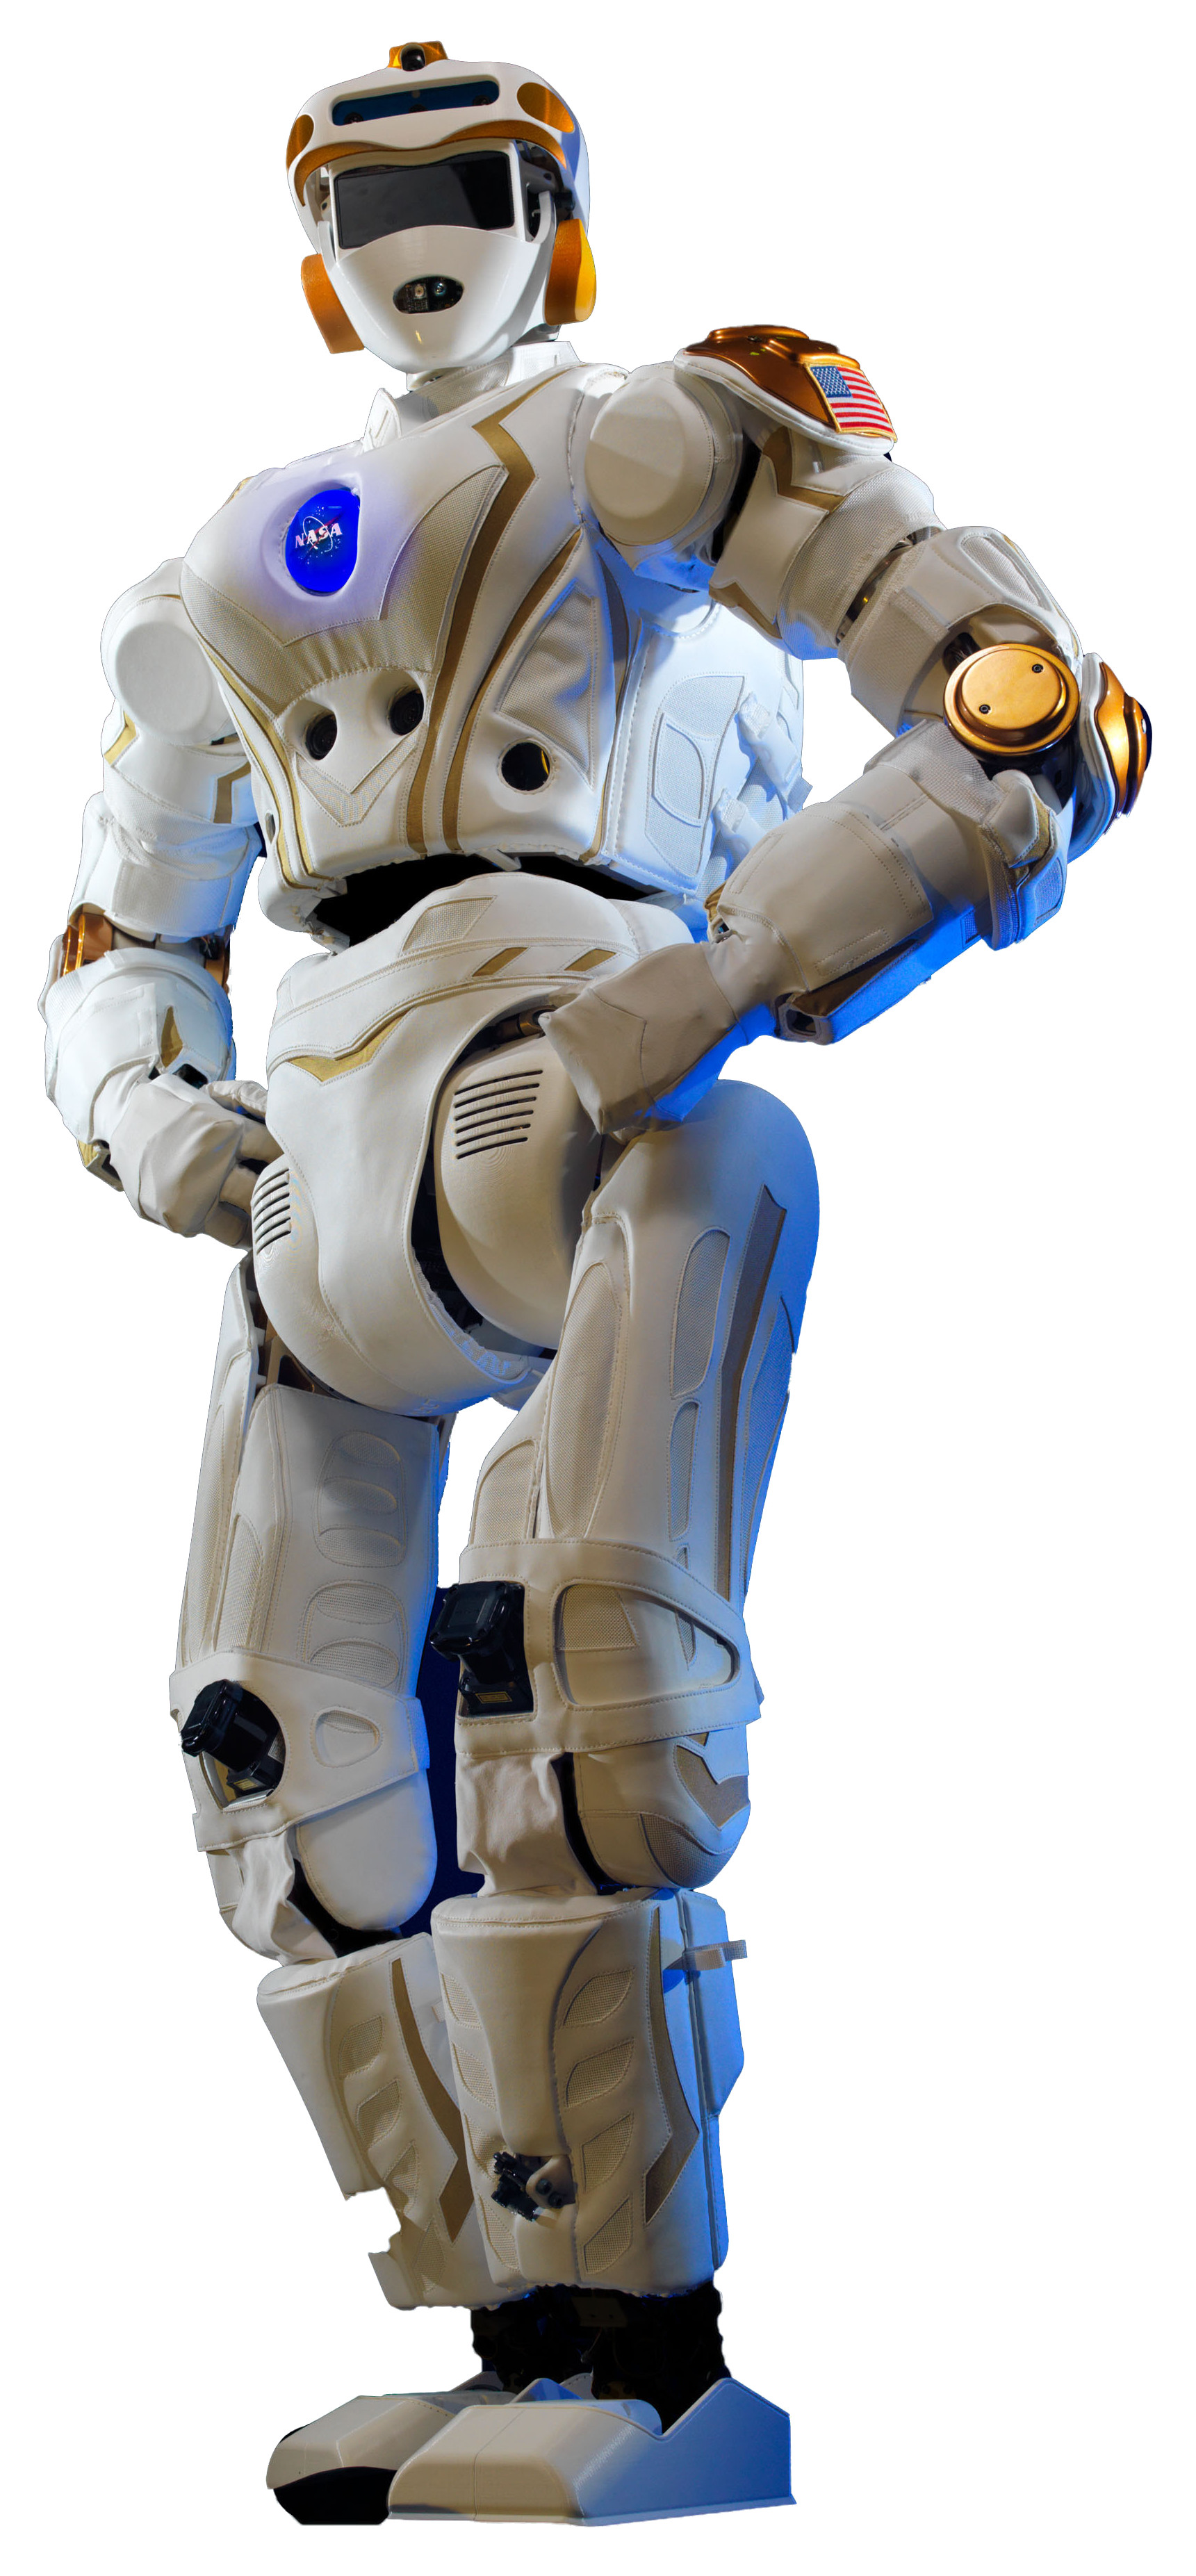
\includegraphics[width=0.6\textwidth]{images/valkyrie/Valkyrie.jpg}
\caption[Valkyrie]{Humanoid robot Valkyrie (Image credits: NASA)}
\label{fig:valkyrie}
\end{minipage}
%
\hspace{0.5cm}
%
\begin{minipage}{0.5\textwidth}
\centering
\subfloat[MultiSense SL]{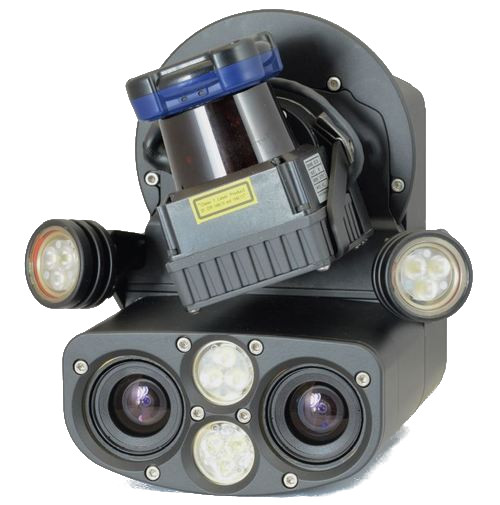
\includegraphics[width=0.8\textwidth]{images/valkyrie/MultiSense_SL.jpg} \label{fig:multisense}}

\subfloat[Asus Xtion PRO]{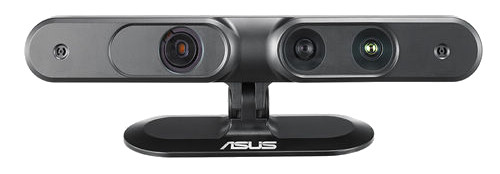
\includegraphics[width=0.8\textwidth]{images/valkyrie/xtion_pro_live.jpg} \label{fig:xtion_pro}}
\caption[Depth sensors]{Depth perception systems (Image credits: (a) Carnegie Robotics, (b) Asus)}
\label{fig:depth_sensors}
\end{minipage}
\end{figure}

The robot will use depth data as its main source of information for estimating the configuration of the manipulator and the object pose. The MultiSense SL stereo and LIDAR depth sensor (\cref{fig:multisense}), which is mounted inside the head of the robot, provides two source of depth image from (1) stereo matching at \SI{15}{\hertz}, and (2) a rotating LIDAR which generates a fill scan at \nicefrac{1}{6} \si{\hertz}. An optional structure from light sensor (\cref{fig:xtion_pro}), which can be mounted on top of the head, uses the known location of projected IR dots to estimate the depth at these locations. The stereo cameras have its IR filter removed to enhance stereo matching by providing distinct keypoints from the IR pattern. The LIDAR data is not applied for tracking because of its low update rate.
The key properties of both depth sensors are compared in \cref{tab:depth_sensor_comparison}. These properties are used to back-project the disparity values into the 3D points.

\begin{table}
\captionsetup{width=0.7\textwidth}
\centering
\begin{tabular}{|c||c|c|}
\hline
 & \textit{MultiSense SL} & \textit{Asus Xtion PRO Live} \\
\hline
\hline
depth range & \SI{0.4}{\meter} - \SI{10}{\meter} & \SI{0.8}{\meter} - \SI{3.5}{\meter} \\
\hline
FOV & \SI{80}{\degree} $\times$ \SI{45}{\degree} & \SI{58}{\degree} $\times$ \SI{45}{\degree} \\
\hline
resolution & $1024 \times 1024$ & $640 \times 480$ \\
\hline
FPS & \SI{15}{\hertz} & \SI{30}{\hertz} \\
\hline
%f & \SI{6.5}{\milli\meter} & • \\
%\hline
$f_x$, $f_y$ & \SI{556.183}{pxl} & \SI{528.014}{pxl} \\
\hline
$c_x$, $c_y$ & \SI{512}{pxl} & (\SI{320}{pxl}, \SI{267}{pxl}) \\
\hline
b & \SI{0.07}{\meter} & \SI{0.075}{\meter} \\
\hline
\end{tabular}
\caption[Comparison of depth sensors]{Comparison of depth sensors. FOV: field of view, FPS: frames per second, $f$: focal length, $c$: image centre, $b$: baseline}
\label{tab:depth_sensor_comparison}
\end{table}


\subsection{Robot Model Representation}

Part of this thesis is the adaptation of the reference implementation to robot model representations stored in the URDF (Unified Robot Description Format) format. URDF defines at a minimum a tree structure that resembles the kinematic tree of a robot with its joints and links. In addition it can provide, among other things, information about joint limits and the geometric properties of the links. These geometric properties can be defined as primitive shapes like spheres, boxes or cylinders, or alternatively refer to complexer triangle meshes.

The URDF plugin for DART is designed that way, that all parts of the kinematic chain that are connected to a given root frame are tracked. This enables us to neglect robot parts that are not involved in manipulation. \cref{fig:val_model_dart} shows such a model that is loaded from the \texttt{torso} frame upwards in the kinematic tree. Hence, it includes both arms, hands and the head with the sensors. This enables us to track both hands in a bi-manual grasping task with respect to the camera frame without invalidating kinematic constraints, such as overrunning joint limits or disconnecting links.

\begin{figure}
\centering
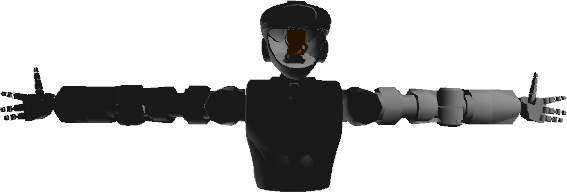
\includegraphics[width=\textwidth]{images/valkyrie/val_model_torso_dart.png}
\caption{Robot model loaded in DART}
\label{fig:val_model_dart}
\end{figure}


\section{Signed Distance Function}

The descriptions in this section of the thesis are based on work by Schmidt et al. \cite{Schmidt2015} that presents the DART algorithm.

The signed distance function (SDF) gives the shortest distance of a point in the observed point cloud to the robot model. It is signed in the sense that the distance is positive if the point lies outside the model, it is negative if the point is inside the model, and it is zero if the point lies exactly on the surface of the model. DART uses two kind of SDFs: the model SDF and the observation SDF.

The model SDF (\cref{fig:model_SDF}) gives the shortest distance of a point to a rigid model mesh. For articulated models, which consist of multiple such model meshes, a local model SDF is applied. This way, the complex computation of a global model SDF for each articulation can be broken down to the parallel computation of local SDF per robot part. For each point in the point cloud data, the distance to each robot part, respectively frame, is computed using the precomputed local SDFs. The point is then associated to the robot frame with the smallest absolute distance value.

In addition to considering observed data and the robot model, which is defined as \textit{positive information} in DART, the optimization is also using \textit{negative information}. If a point is observed in 3D, there cannot be anything in between this point and the camera centre. This free space constrain is visualised in \cref{fig:observation_SDF}. This observation SDF uses the distance transform on the observation and the estimated configuration of the model from the model SDF to constrain models to not be in free space.

\begin{figure}
\centering
\subfloat[Model SDF]{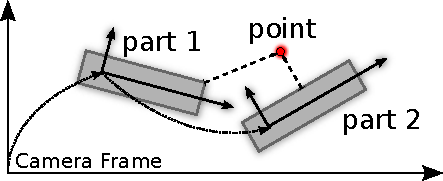
\includegraphics[width=0.5\textwidth]{images/sdf/local_sdf.pdf} \label{fig:model_SDF}}
\subfloat[Observation SDF]{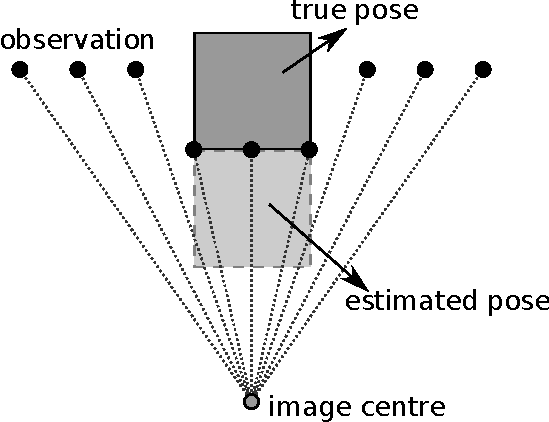
\includegraphics[width=0.3\textwidth]{images/sdf/sdf_obs.pdf} \label{fig:observation_SDF}}
\caption[Signed Distance Function]{Local model SDF and observation SDF (Inspired by \cite{Schmidt2015} figures 3 and 6). (a) the observed point is assigned to \emph{part 2}, (b) the estimated box (light gray) lies in between the observation and the image centre and thus invalidates the free space constrain.}
\end{figure}

\section{Gauss-Newton Algorithm}

The \textit{Gauss-Newton} algorithm is a method for finding the optimal set of parameters $\mathbf{p}$ that minimizes the sum of squares of non-linear vector-valued objective functions $e(\cdot)$
%
\begin{equation}
\hat{\mathbf{p}} = \arg\min_{p} \sum_{i=1}^N\left[ e_i(\mathbf{p})^2\right] .
\end{equation}

The Gauss-Newton algorithm is derived from the \textit{Newton} algorithm for finding roots and extremal points which itself is based on the Taylor series expansion. The Newton method for finding extremal points of the scalar objective function $f(x)$ is an iterative procedure
%
\begin{equation}
x_{t+1} = x_t - \frac{f^{(1)}(x_t)}{f^{(2)}(x_t)}
\label{eqn:newton_minimum}
\end{equation}
%
starting at an initial state $x_0$ using the first- and second-order derivatives ($f^{(1)}$, $f^{(2)}$) of the objective function.

For finding the minimum of the function $e(\cdot)$ with respect to a parameter vector $\mathbf{p}$, the first- and second-order partial derivatives are used. In particular, the first- and second-order derivatives in \ref{eqn:newton_minimum} are replaced by the gradient $\nabla e(\mathbf{p})$ and the Hessian $\nabla^2 e(\mathbf{p})$ of the objective function $e$.
The partial derivatives of the vector-valued function $e(\cdot)$ with respect to the parameter vector $\mathbf{p}$ are aggregated in the \textit{Jacobian} matrix $J\in \mathbb{R}^{i \times j}$ with elements
%
\begin{equation}
J_{i,j} = \frac{\partial e_i(\mathbf{p})}{\partial p_j} .
\end{equation}
%
Hence,
\begin{align}
\nabla e(\mathbf{p}) &= J^\top e(\mathbf{p}) \label{eqn:gn_gradient}\\
H(e) = \nabla^2 e(\mathbf{p}) &= J^\top J +  \sum_{i=1} e_i(\mathbf{p}) \nabla^2 e_i(\mathbf{p}) \label{eqn:gn_hessian_full}.
\end{align}

For small $e$, the Hessian $H(e)$ can be approximated by
\begin{equation}
H(e) \approx J^\top J \label{eqn:gn_hessian}
\end{equation}
%
neglecting the second-order derivatives. This approximation is used in the Gauss-Newton algorithm and the parameter update step becomes
%
\begin{align}
\mathbf{p}_{t+1} &= \mathbf{p}_{t} - \Delta\mathbf{p} \\
&= \mathbf{p}_{t} - H(e)^{-1} \cdot \nabla e(\mathbf{p}) \\
&= \mathbf{p}_{t} - \left(J^\top J\right)^{-1} \cdot J^\top e(\mathbf{p}) \label{eqn:gn_param_update}.
\end{align}

The parameter update $\Delta\mathbf{p}$ is proportionally driven by the gradient of the objective function and inverse proportional by the approximation of the Hessian.


\section{Prior Information}

Prior information can be used in the Gauss-Newton algorithm by modulating the Hessian approximation and the gradient towards the desired state. This is achieved by selecting an objective function and calculating its partial derivatives with respect to the parameter vector. These partial derivatives are used in the Jacobian as shown in equations \ref{eqn:gn_gradient} and \ref{eqn:gn_hessian}.

The full parameter vector in DART consists of the 6D pose of the root frame and the $N$ joints positions:
\begin{equation}
\mathbf{p} = \begin{bmatrix}
x & y & z & \phi & \theta & \psi & | & q_1 & \cdots & q_N
\end{bmatrix}
\end{equation}

with $x$, $y$, $z$ for the translation, $\phi$, $\theta$, $\psi$ for the orientation in radiant Euler angles, and $q_1 \dots q_N$ the individual joint position values.


\subsection{Known Frame Pose}

For constraining the translation of the root frame in between optimization iterations, the parameter update vector $\Delta\mathbf{p}$ must be computed such that its first 6 elements for the pose are $0$. From equation \ref{eqn:gn_param_update}
\begin{align}
\Delta\mathbf{p} &= \left(J^\top J\right)^{-1} \cdot J^\top e(\mathbf{p}) = \begin{bmatrix}
\mathbf{0} & | & q_1 & \cdots & q_N
\end{bmatrix} \\
J^\top e &= J^\top J \cdot \begin{bmatrix}
\mathbf{0} & | & q_1 & \cdots & q_N
\end{bmatrix}
\end{align}

Cancelling out the pose update can be achieved by applying the prior on the final blended Hessian and gradient just before the final parameter update is computed. In particular the fixed frame prior computes the parameter update $\Delta\mathbf{p}$ from the blended Hessian and gradient, cancels out the first 6 elements for the pose, and computes the new gradient. Instead of blending this gradient ($J^\top e$) into the final gradient, the global gradient is overwritten resulting in enforcing no frame pose update.


\subsection{Reported Joint Positions}

We use the reported state of the robot in a way, that we can drag the estimated solution away from possibly distracting perceptions towards the state perceived through the joint encoders.
%
Three different kind of objective functions have been selected for this purpose which compute a weighted deviation of the estimated joint configuration $\mathbf{q}$ from reported joint configuration $\mathbf{r}$. For all objective functions, $r_i$ and $q_i$ denote the individual joint positions in their corresponding configuration vector.

\begin{enumerate}
\item Weighted L2 norm of the estimated joint position deviation:
\begin{equation}
e_1 = w \cdot \lVert \mathbf{r} - \mathbf{q} \rVert = w \cdot \sqrt{\sum_{i=1}^N (r_i - q_i)^2} \label{eqn:objf_weightedL2}
\end{equation}
with scalar weight $w>0$.

\item L2 norm of the weighted joint deviation:
\begin{equation}
e_2 = \lVert w \cdot (\mathbf{r} - \mathbf{q}) \rVert = \sqrt{\sum_{i=1}^N w \cdot (r_i - q_i)^2} \label{eqn:objf_L2ofweighted}
\end{equation}
with the same scalar weight $w>0$ for all joint deviations.

\item Sum of squares of individually weighted joints:
\begin{equation}
e_3 = \lvert \mathbf{r} - \mathbf{q} \rvert^\top Q \lvert \mathbf{r} - \mathbf{q} \rvert = \sum_{i=1}^N \left[ (r_i-q_i) \cdot \sum_{j=1}^N (r_j-q_j) \cdot \omega_{i,j} \right] \label{eqn:objf_indiv_weighted}
\end{equation}
with the weight matrix $Q\in\mathbf{R}^{N\times N}$ and its elements $\omega_{i,j}$. As a error metric, the weight matrix $Q$ must be \emph{positive-semidefinite}. That is, $\forall \mathbf{x}\in\mathbf{R}^n: x^\top Q x \geq 0$.
\end{enumerate}

Whereas the first two objective functions (\ref{eqn:objf_weightedL2} and \ref{eqn:objf_L2ofweighted}) use a common scalar weight for all joint deviations, the third objective function (\ref{eqn:objf_indiv_weighted}) can apply different weights per joint and hence enables to penalize whole parts of the kinematic chain more precise.

The respective partial derivatives for the Jacobian are:
\begin{enumerate}
\item Weighted L2 norm of the estimated joint position deviation
\begin{equation}
J_{ji} = \frac{\partial e_1}{\partial q_i} = -w \frac{r_i - q_i}{\lVert \mathbf{r} - \mathbf{q} \rVert}
\end{equation}

\item L2 norm of the weighted joint deviation:
\begin{equation}
J_{ji} = \frac{\partial e_2}{\partial q_i} = -w^2 \frac{r_i - q_i}{\lVert w \cdot (\mathbf{r} - \mathbf{q}) \rVert}
\end{equation}

\item Sum of squares of individually weighted joints:
\begin{equation}
J_{ji} = \frac{\partial e_3}{\partial q_i} = - \left[ \sum_{j=1}^N d_jq_{i,j}\right] + \left[ \sum_{j=1 \neq i}^N d_jq_{j,i}\right]
\end{equation}
\end{enumerate}


\section{Ground Truth Data Collection}

To evaluate the tracking performance and verify the effect of the joint position prior, reference measurements of the true state of the robot are required. The Vicon motion caption system is selected to externally track the pose of IR reflective markers rigidly attached to the robot.

\subsection{Setup}

To obtain the true transformation from the pelvis frame to the left hand palm frame, reflective markers are rigidly mounted with standoffs to the specific robot frames. The photograph in \cref{fig:vicon_marker} shows the highlighted location of the markers on the \texttt{pelvis} frame (green) and the \texttt{leftPalm} frame (red).

\begin{figure}
\captionsetup{width=0.4\textwidth}
\centering
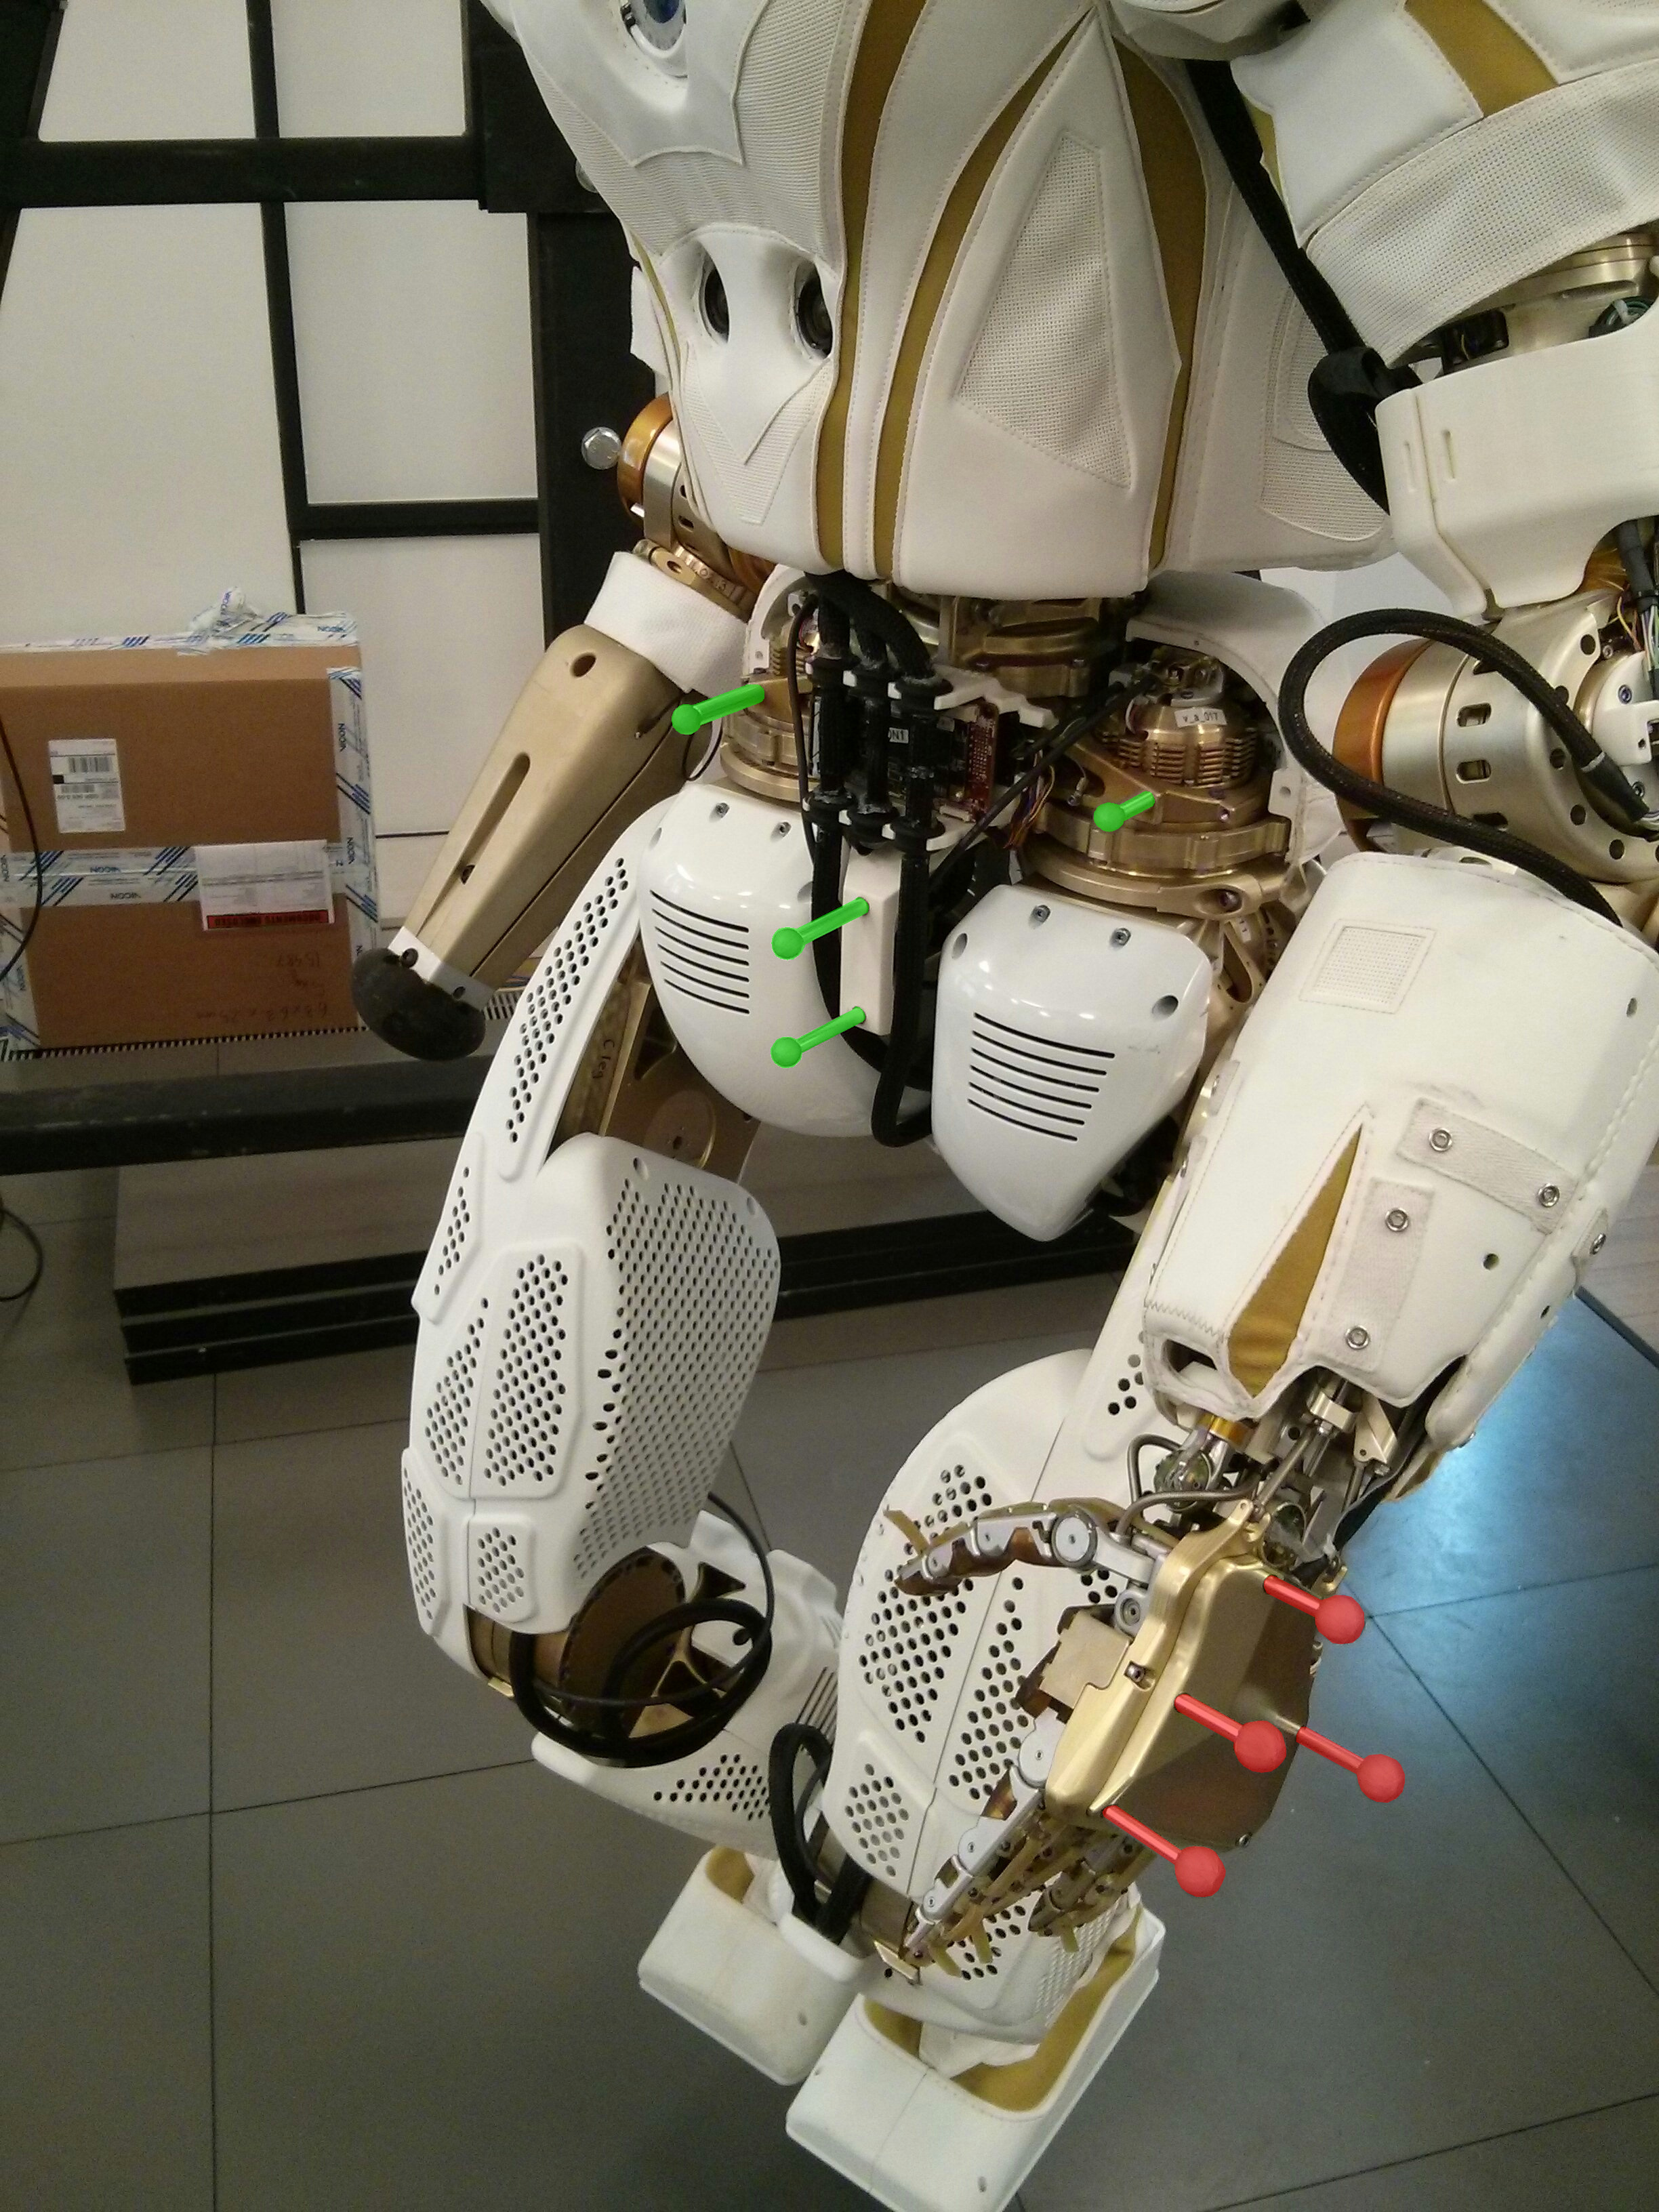
\includegraphics[width=0.4\textwidth]{images/vicon_pose/vicon_marker_col.jpg}
\caption[Location of Vicon marker]{Location of Vicon marker on pelvis (green) and left hand (red)}
\label{fig:vicon_marker}
\end{figure}


\subsection{Hand Pose}

Each group of markers has its own coordinate system with its origin in the centre.
The drawing in \cref{fig:transform_vicon_robot} visualizes the transformations between the Vicon world frame, the Vicon marker frames and the robot frames.
The transformations $T_{w \rightarrow vp}$ and $T_{w \rightarrow vh}$ are the reported poses of the Vicon marker in the world frame.
To obtain the transformation $T_{p \rightarrow h}$, which gives the hand pose in the pelvis frame, we need to find the rigid transformation between the Vicon marker and robot frame ($T_{m \rightarrow p}$ and $T_{m \rightarrow h}$).

\begin{figure}
\captionsetup{width=0.52\textwidth}
\centering
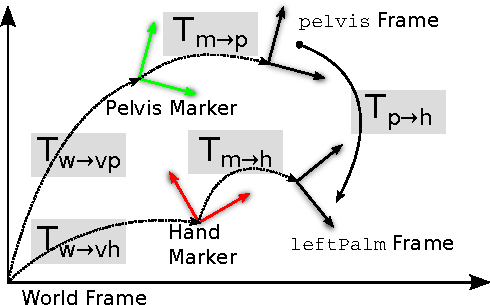
\includegraphics[width=0.5\textwidth]{images/vicon_pose/vicon_transforms.pdf}
\caption[Transformations of Vicon markers]{Transformations between Vicon markers (\textit{pelvis} - green, \textit{hand} - red) and robot frames}
\label{fig:transform_vicon_robot}
\end{figure}

The rigid transformation between marker and robot frames can be obtained by a least-squares optimization on corresponding points in both frames \cite{Umeyama1991}. Given corresponding points $m_i$ in marker frame and $x_i$ in the robot frame, the optimal projection of marker points from the marker frame into corresponding points in the robot frame becomes
\begin{equation}
T_{x \rightarrow m} = \arg\min_{R,t} \frac{1}{N} \sum_{i=1}^N \lVert x_i - \left( R \cdot m_i + t \right) \rVert_2
\label{eqn:least_squares_transformation_estimation}
\end{equation}
where $T_{x \rightarrow m}$ denotes the homogeneous transformation matrix containing the rotation matrix $R$ and the translation vector $t$. The points $x_i$ in the robot frame are here interchangeable for points $p_i$ in the \texttt{pelvis} frame and $h_i$ in the \texttt{leftPalm} frame.

%The Vicon system provides the pose of the marker frame in the world coordinate frame. That is the inverse of the transformations $T_{w \rightarrow vp}^{-1}$ and $T_{w \rightarrow vh}^{-1}$, e.g. the projection of the marker into the world frame.
The pose of the \texttt{pelvis} and \texttt{leftPalm} frame in the Vicon world frame can be expressed by the transformations
\begin{align}
T_{w \rightarrow p} &= T_{w \rightarrow vp} \cdot T_{p \rightarrow m} = T_{w \rightarrow vp} \cdot T_{m \rightarrow p}^{-1} \\
T_{w \rightarrow h} &= T_{w \rightarrow vh} \cdot T_{h \rightarrow m} = T_{w \rightarrow vh} \cdot T_{m \rightarrow h}^{-1} .
\end{align}

The transformations between these robot frames then finally becomes
\begin{align}
T_{w \rightarrow h} &= T_{w \rightarrow p} \cdot T_{p \rightarrow h} \\
T_{w \rightarrow vh} \cdot T_{m \rightarrow h}^{-1} &= T_{w \rightarrow vp} \cdot T_{m \rightarrow p}^{-1} \cdot T_{p \rightarrow h} \nonumber \\
T_{p \rightarrow h} &= \left( T_{w \rightarrow vp} \cdot T_{m \rightarrow p}^{-1} \right)^{-1} \cdot T_{w \rightarrow vh} \cdot T_{m \rightarrow h}^{-1} \label{eqn:hand_pose_from_vicon} .
\end{align}

Given the transformations of the Vicon markers ($T_{w \rightarrow vp}$ and $T_{w \rightarrow vh}$) at each time instance, and the rigid transformation between these markers and the robot frame ($T_{m \rightarrow p}$ and $T_{m \rightarrow h}$) we can recover the true pose of the hand in the pelvis frame ($T_{p \rightarrow h}$) using \cref{eqn:hand_pose_from_vicon}.


\subsection{Joint Position Offset Calibration}

The availability of a true transformation within the robot kinematic chain enables us to compare the reported hand pose from forward kinematics with the true hand hand pose and further, calibrate the joints in the kinematic chain such that this deviation is minimized.

For minimizing the joint position deviation and obtaining correction offsets, the same optimization approach as described in \cite{Fallon2015} is applied. That is, given a correction function that maps a reported joint position value to its corrected value: $f_{corr}: q_{rep,i} \mapsto q_{corr,i}$, and a mapping from this joint space configuration to the 	task space pose of the manipulator using forward kinematics $\phi: \mathbf{q} \mapsto \mathbf{p}$, with the pose $\mathbf{p} \in SE(3)$, the optimal correction parameters can be found by minimising
\begin{equation}
e = \frac{1}{N} \sum_{i=1}^N  \lVert \phi \left( f_{corr}(q_{rep,i}) \right) - \mathbf{p}_i \rVert_2
\end{equation}
for $N$ samples, respectively poses. The average error is selected over the summed error to have comparable costs between varying lengths of sample sequences.

Two correction function $f_{corr}$ have been selected. The constant correction
\begin{equation}
f_{corr}(q_{rep}) = q_{offset} + q_{rep}
\end{equation}
assumes constant offset that is independent from the reported joint position value itself. Here, only one parameter per calibrated joint is to be optimized. A linear correction function
\begin{equation}
f_{corr}(q_{rep}) = q_{offset} + m_1 \cdot q_{rep}
\end{equation}
assumes an additional relation to the reported joint position value itself. In this case twice the parameters are optimised.

To prevent overfitting of the optimized correction parameters on the data set, the optimization result must be applied to a dedicated test set that has not been used for optimization. This is especially the case for more complex correction functions.

\chapter{Evaluation}
\label{sec:evaluation}

The articulated tracking approach and the incorporation of prior information is evaluated on two different data sets. The data set for the \textit{first experiment} contains depth observations from a manipulator that is moving close to a table and an object. This experiment will be used to compare different approaches to incorporate prior information in the tracking process.

The data set for the \textit{second experiment} contains stereo camera observations of the manipulator at different viewing angles without nearby objects. This data set additionally contains the ground truth hand pose that were measured by the Vicon system.

\section{Experiment 1: Incorporating Prior Information}

This section will evaluate the application of prior information in a setting where a robot hand moves close to an object and a table. Two sources of depth information are considered: enhanced stereo matching using IR dot projection (denoted as \emph{stereo}) and structured light (denoted as \emph{xtion} as in Asus Xtion).

\subsection{Hypotheses}

In the base implementation of the assessed tracking approach, its gradient is determined by the signed distance function. Hence, the optimization is driven by the observation once the iteration is initialized with the reported state. Using additional information that effects the gradient can improve the state estimation by driving it away from distracting observations.

\begin{hypothesis}(Distracting sensor readings)\\
Distracting sensor readings will impair the tracking performance of the manipulator.
\label{hyp:distracting_readings}
\end{hypothesis}

\begin{hypothesis}(Use of prior information)\\
Using prior information will reduce the negative effects of distracting sensor readings. Increasing weights will further decrease the dependency on the sensor readings.
\label{hyp:prior_information}
\end{hypothesis}


\subsection{Setup}

A robot was placed in front of a table with a bottle on it. The left hand was moved from close to the table plane towards the object. Once the object is pushed, the hand moved up and back to its initial position.
The setup, as it is perceived by the robots stereo vision in the initial state, is shown in \cref{fig:exp1_setup}.

%\begin{figure}
%\centering
%\begin{minipage}{0.45\textwidth}
%\centering
%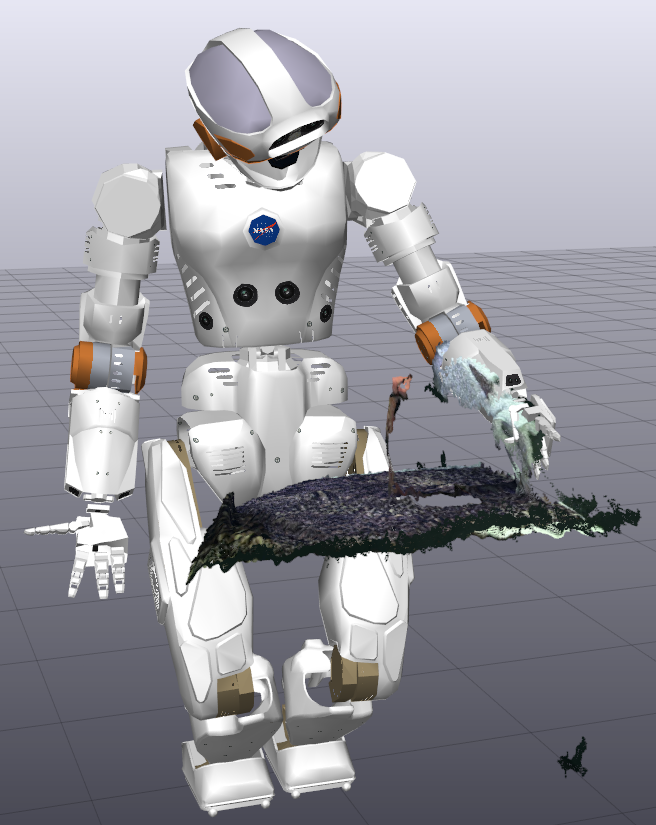
\includegraphics[width=1.0\textwidth]{images/eval_prior/sequence/prior_setting.png} 
%\caption{Joint prior setup}
%\label{fig:prior_setting}
%\end{minipage}
%%
%\hspace{0.3cm}
%\begin{minipage}{0.45\textwidth}
%\vspace{0.8cm}
%\centering
%\subfloat[start (t=0)]{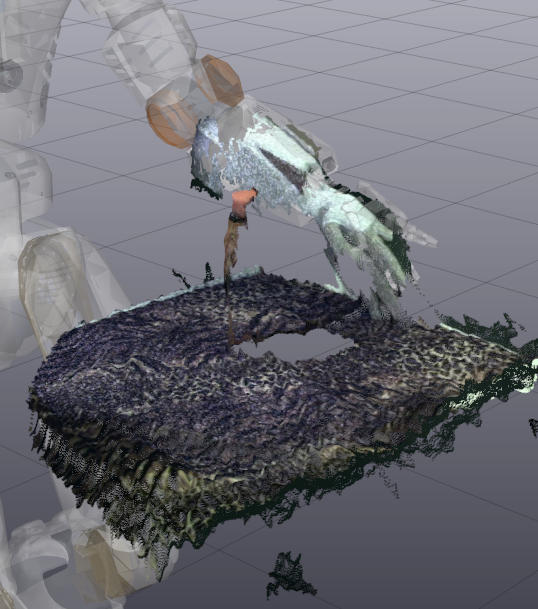
\includegraphics[width=0.5\textwidth]{images/eval_prior/sequence/bottle_0_init.png} \label{fig:prior_movement_phases_start}}
%\subfloat[moved upwards (t=10)]{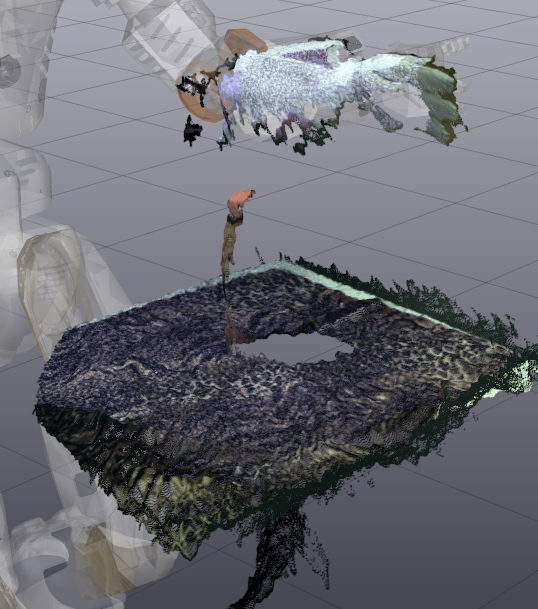
\includegraphics[width=0.5\textwidth]{images/eval_prior/sequence/bottle_10_up.png} }
%
%\subfloat[object contact (t=22)]{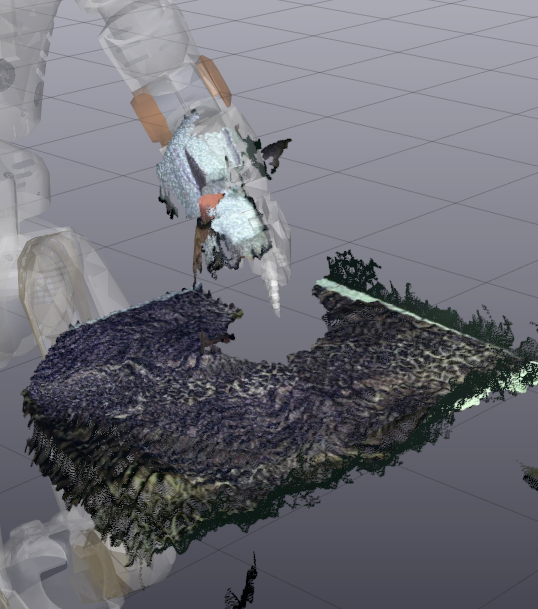
\includegraphics[width=0.5\textwidth]{images/eval_prior/sequence/bottle_22_object.png} 
%\label{fig:prior_movement_phases_contact}}
%\subfloat[end (t=35)]{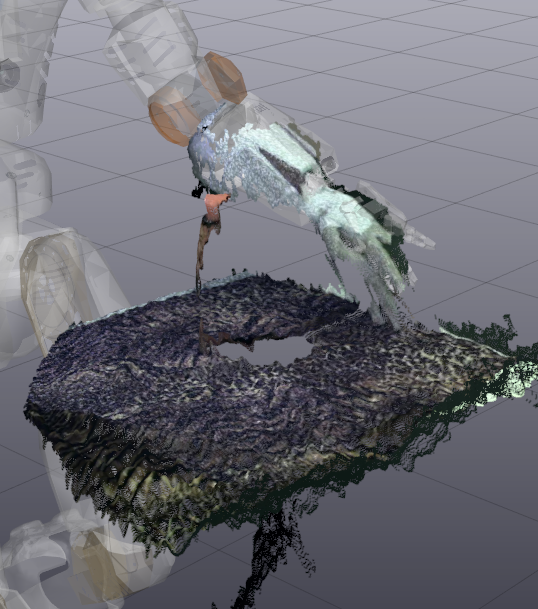
\includegraphics[width=0.5\textwidth]{images/eval_prior/sequence/bottle_35_end.png} }
%\caption[States between movements]{Sequence of states between movements (time in seconds)}
%\label{fig:prior_movement_phases}
%\end{minipage}
%\end{figure}


\begin{figure}[h]
\centering
\subfloat[Point cloud and reported robot state]{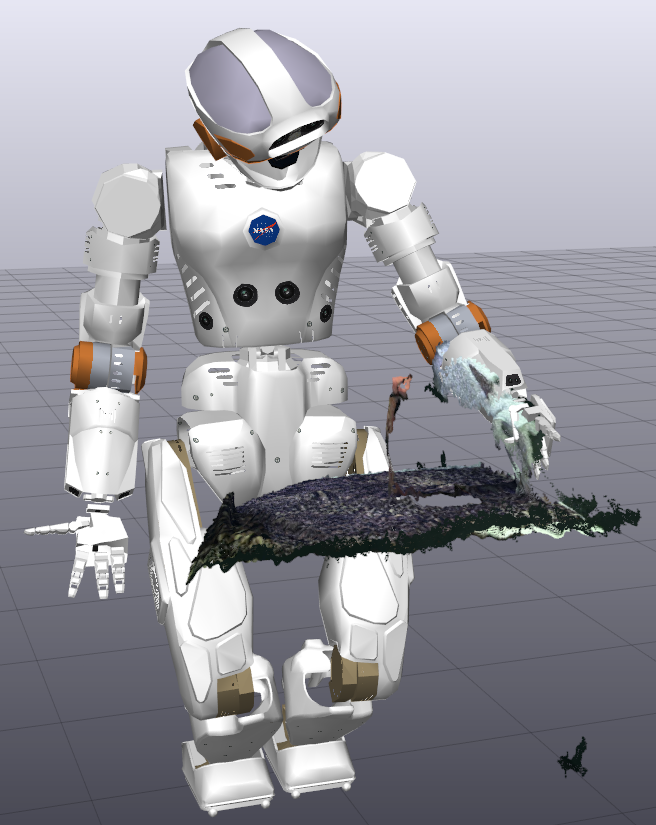
\includegraphics[height=7cm]{images/eval_prior/sequence/prior_setting.png} }
\hspace{1cm}
\subfloat[View from left camera]{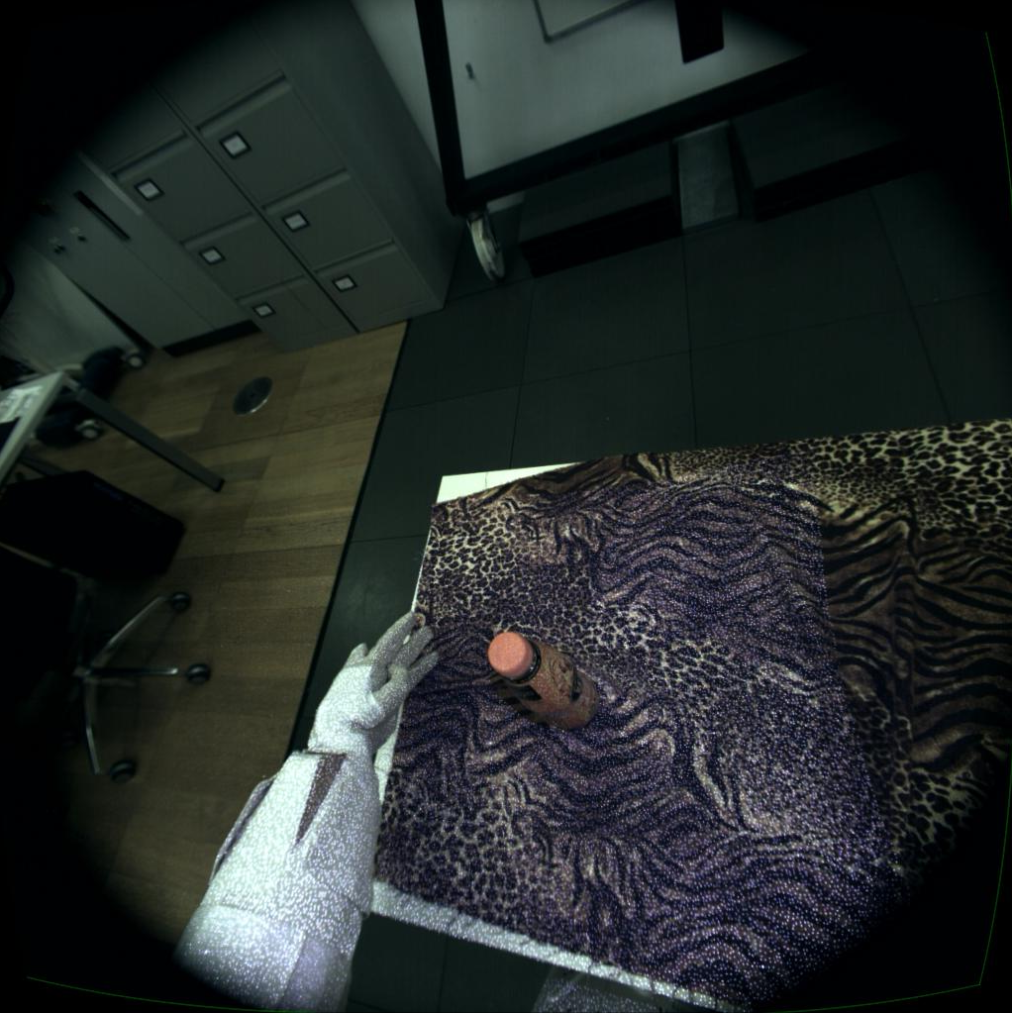
\includegraphics[height=7cm]{images/eval_prior/sequence/camera_view_initial.png} }
\caption[Experiment 1: Setup]{Experiment 1: Setup with robot in front of table. Initial state where manipulator is observed close to table plane.}
\label{fig:exp1_setup}
\end{figure}

The motion sequence is divided into 5 states which change by 4 movements. The movement phases are defined in \cref{tab:prior_movement_phases}. Two of the phases define movements of the manipulator away from objects after being in contact with them. These phases are highlighted in the table and in the plots.

\begin{table}[h]
\centering
\begin{tabular}{|c|l|l|}
\hline
 & \emph{time (s)} & \emph{movement description} \\
\hline
1 & 0$\dots$3 & arm resting on table \\
\hline
\rowcolor{gray!30} \textbf{2} & 3$\dots$10 & upward from table \\
\hline
3 & 10$\dots$20 & towards object \\
\hline
\rowcolor{gray!30} \textbf{4} & 20$\dots$30 & away from object \\
\hline
5 & 30$\dots$35 & downward towards table \\
\hline
\end{tabular}
\caption{Phases of arm movement in experiment 1. Highlighted rows emphasise movements away from objects like the table or bottle.}
\label{tab:prior_movement_phases}
\end{table}

The perceived point cloud of the first three states and the final state are shown in \cref{fig:prior_movement_phases}.
Especially the movement phases 2 and 4, respectively movements starting in states shown in \cref{fig:prior_movement_phases_start,fig:prior_movement_phases_contact} are of interest.

\begin{figure}[h]
\centering
\subfloat[start (t=0)]{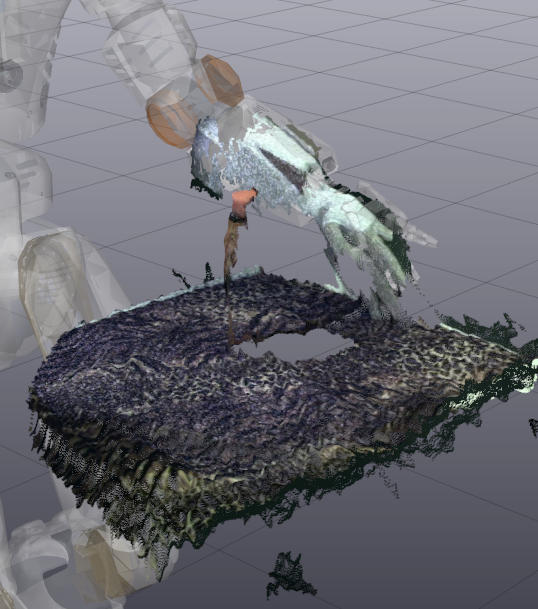
\includegraphics[width=0.25\textwidth]{images/eval_prior/sequence/bottle_0_init.png} \label{fig:prior_movement_phases_start}}
\subfloat[moved upwards (t=10)]{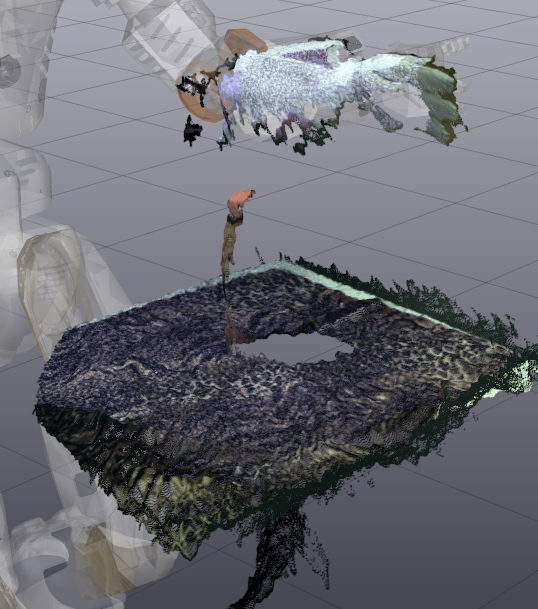
\includegraphics[width=0.25\textwidth]{images/eval_prior/sequence/bottle_10_up.png} }
\subfloat[object contact (t=22)]{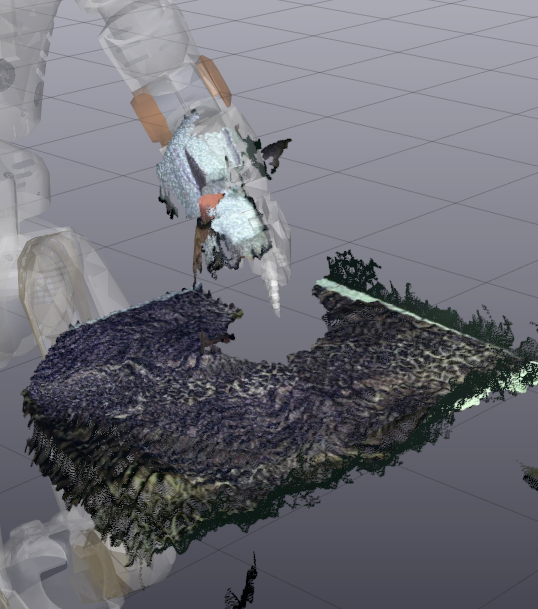
\includegraphics[width=0.25\textwidth]{images/eval_prior/sequence/bottle_22_object.png} 
\label{fig:prior_movement_phases_contact}}
\subfloat[end (t=35)]{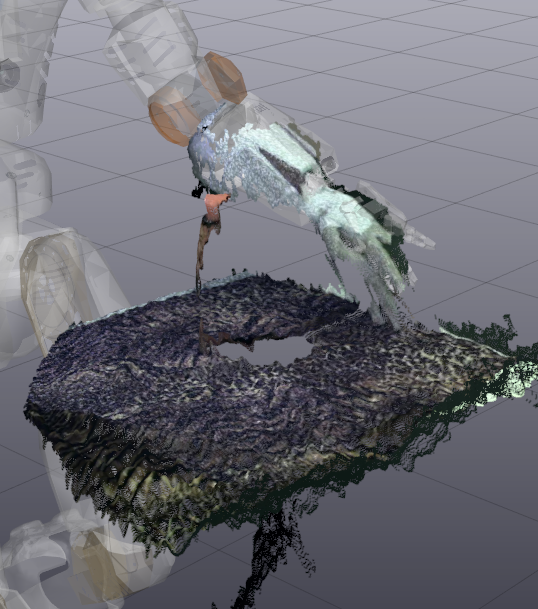
\includegraphics[width=0.25\textwidth]{images/eval_prior/sequence/bottle_35_end.png} }
\caption[Experiment 1: States between movements]{Sequence of states between movements in experiment 1 (time in seconds)}
\label{fig:prior_movement_phases}
\end{figure}

During the movement, depth data is collected simultaneously from the MultiSense stereo sensor and the Asus Xtion structured light sensor. Hence, the stereo block matching benefits from the distinctive IR dots.


\subsection{Results}
\label{sec:prior_results}

For this experiment, we are interested in the deviation of the estimated state from the reported state. This will allow us to (1) see how the estimation on the observed point cloud is deviating from its initial reported pose, and (2) investigate the effect of the prior objective compared to the base signed distance objective. We will refer to this deviation as \emph{error}.

The error in joint and task space is computed as L2 norm (Euclidean distance) of its components and plotted over time. In joint space these components are the left fingers (13 DoF: 3 $\times$ \emph{leftIndexFingerPitch}, 3 $\times$ \emph{leftMiddleFingerPitch}, 3 $\times$ \emph{leftPinkyPitch}, 3 $\times$ \emph{leftThumbPitch} and 1 $\times$ \emph{leftThumbRoll}) and the left arm (7 DoF: \emph{leftShoulderPitch/Roll/Yaw}, \emph{leftElbowPitch}, \emph{leftForearmYaw}, \emph{leftWristRoll/Pitch}). In task space, the 3D position ($x,y,z$) and the 3D orientation (\textit{roll}, \textit{pitch}, \textit{yaw}) of the left hand (frame: \emph{leftPalm}) are computed via forward kinematics on the reported and estimated robot configuration.

\subsubsection{Joint Prior Objective with Common Weight}

The following plots compare the joint and task space errors for the two depth sources for common weights in the range 0 to 5. The common weighting scheme \emph{Weighted L2 norm of joint position deviation} (objective function \cref{eqn:objf_weightedL2}) is applied. A weight of 0 indicates that no prior is used at all.

\paragraph{Stereo}

\Cref{fig:stereo_joint_error} compares the joint space error for left fingers and arm. For both parts, after the optimization reaches the steady state, the maximum error is reached when no prior information from the reported configuration is used. In this case, the configuration is solely optimized using the distance to the observed point cloud. If the manipulator is close to a large concentration of points, the optimization will relate these readings to the manipulator (\cref{fig:no_prior_fingers_table}).
The general trend is that the error decreases with increasing weight. This is not true for the arm movement in the second half of phase 4 ($t=[20,30]$), where weights of $0.2$ and $0.5$ result in larger errors compared to no prior.

The largest decrease in error can be seen for the finger joints when using already a small weight of $0.2$. A similar effect is not present for the arm joints. This is presumably because the robot can only observe the lower part of its arm and hence the arm configuration is mostly determined by its initial state close to the reported state.

\begin{SCfigure}
\centering
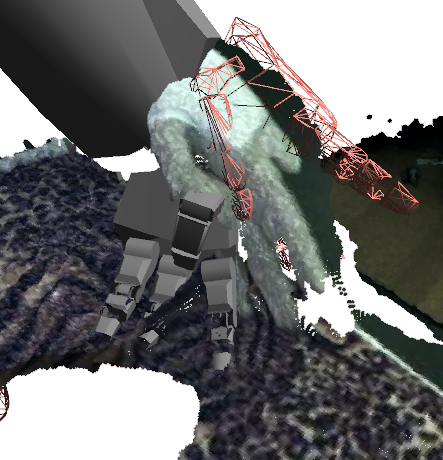
\includegraphics[width=0.5\textwidth]{images/eval_prior/fingers_in_table.png}
\caption[Wrong association of data points]{Close points from the table plane are associated to the fingers (solid gray mesh). Using solely the signed distance as objective, the gradient based optimization finds a local minimum in regions with dense sensor readings close the initial reported state (red wired mesh).}
\label{fig:no_prior_fingers_table}
\end{SCfigure}

\begin{figure}[h]
\centering
\subfloat[finger joints]{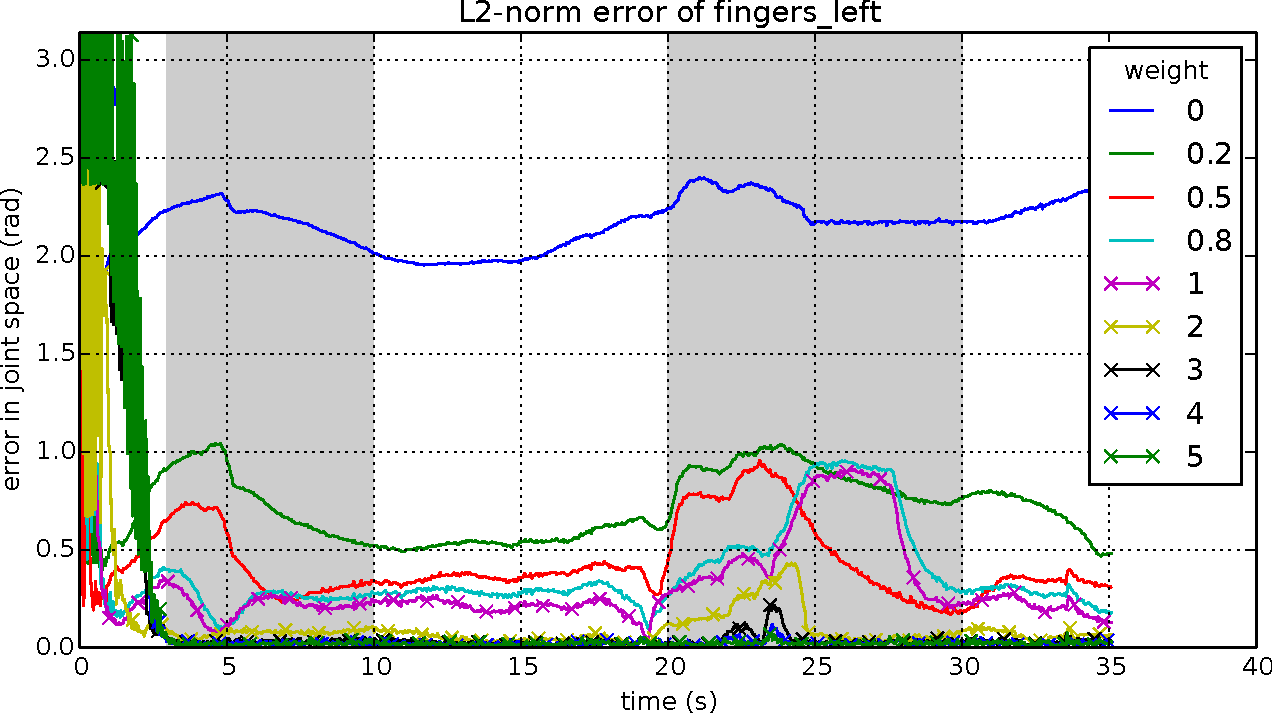
\includegraphics[width=0.5\textwidth]{images/eval_prior/common_weights/stereo_finger_joint_error.pdf} \label{fig:stereo_joint_error_hand} }
%
\subfloat[arm joints]{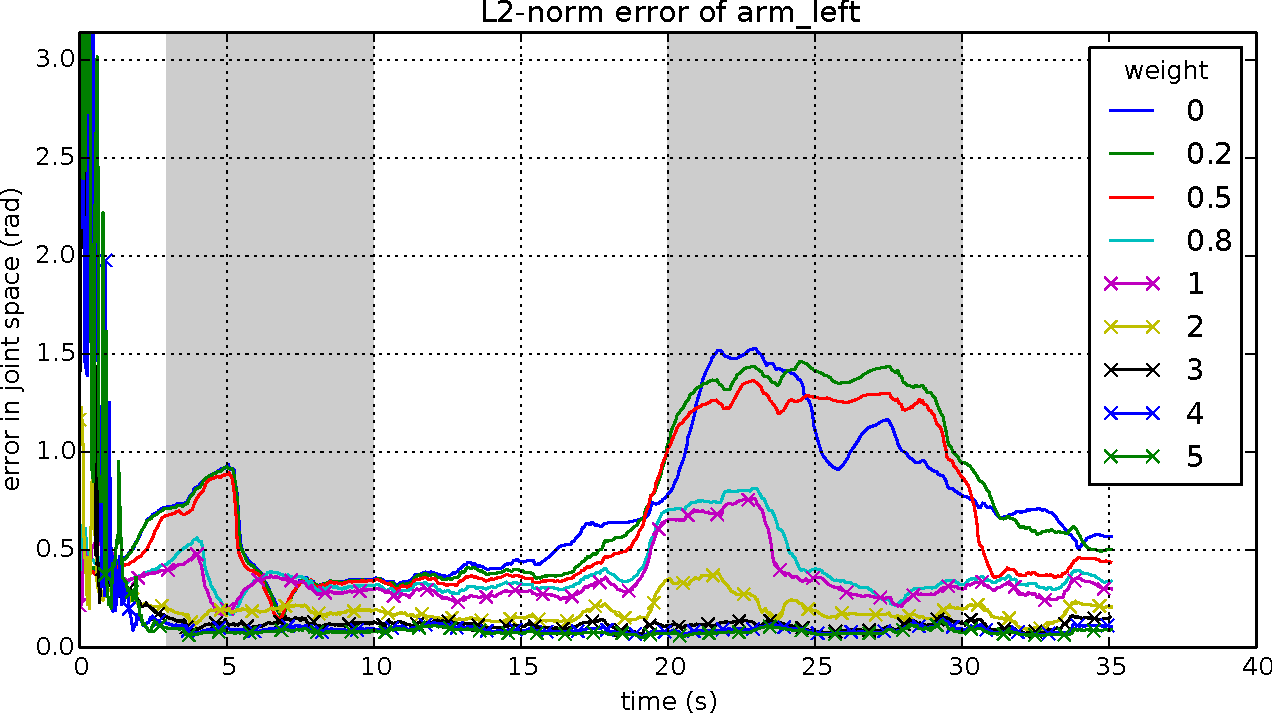
\includegraphics[width=0.5\textwidth]{images/eval_prior/common_weights/stereo_arm_joint_error.pdf} \label{fig:stereo_joint_error_arm} }
\caption[Joint space error (Exp. 1, stereo)]{Joint space error for finger and arm joints (Exp. 1, \textit{stereo} data). The finger joint deviation (a) can already reduces by a weak bias towards the reported pose ($0.2$, $0.5$), while the arm joints (b) require a higher weight ($\geq0.8$).}
\label{fig:stereo_joint_error}
\end{figure}

As the hand position and orientation only depends on the arm configuration but not the finger configuration, we expect some relation between the joint error of the arm and the pose error on the hand frame. We can see this relation, when comparing the joint space error for the arm in \cref{fig:stereo_joint_error_arm} and the hand pose error in \cref{fig:stereo_hand_pose_error}. In particular the error increases in phases where the hand moves upwards and when it moves away from the object (phases 2 and 4). The position error can be reduced significantly when using a prior with low weight ($0.2$), whereas the orientation error reduces only when using prior weights larger or equal than $0.8$.

\begin{figure}[h]
\centering
\subfloat[position error]{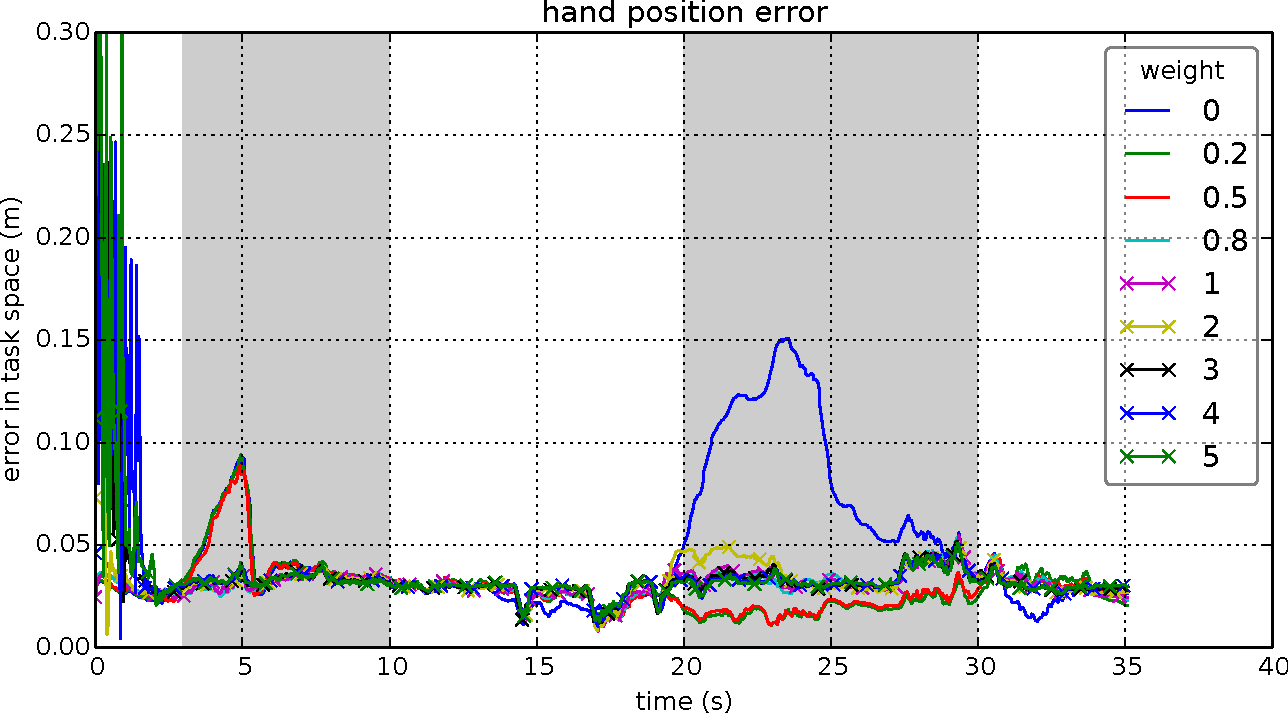
\includegraphics[width=0.5\textwidth]{images/eval_prior/common_weights/stereo_hand_pos_error.pdf} \label{fig:stereo_hand_pos_error}}
%
\subfloat[orientation error]{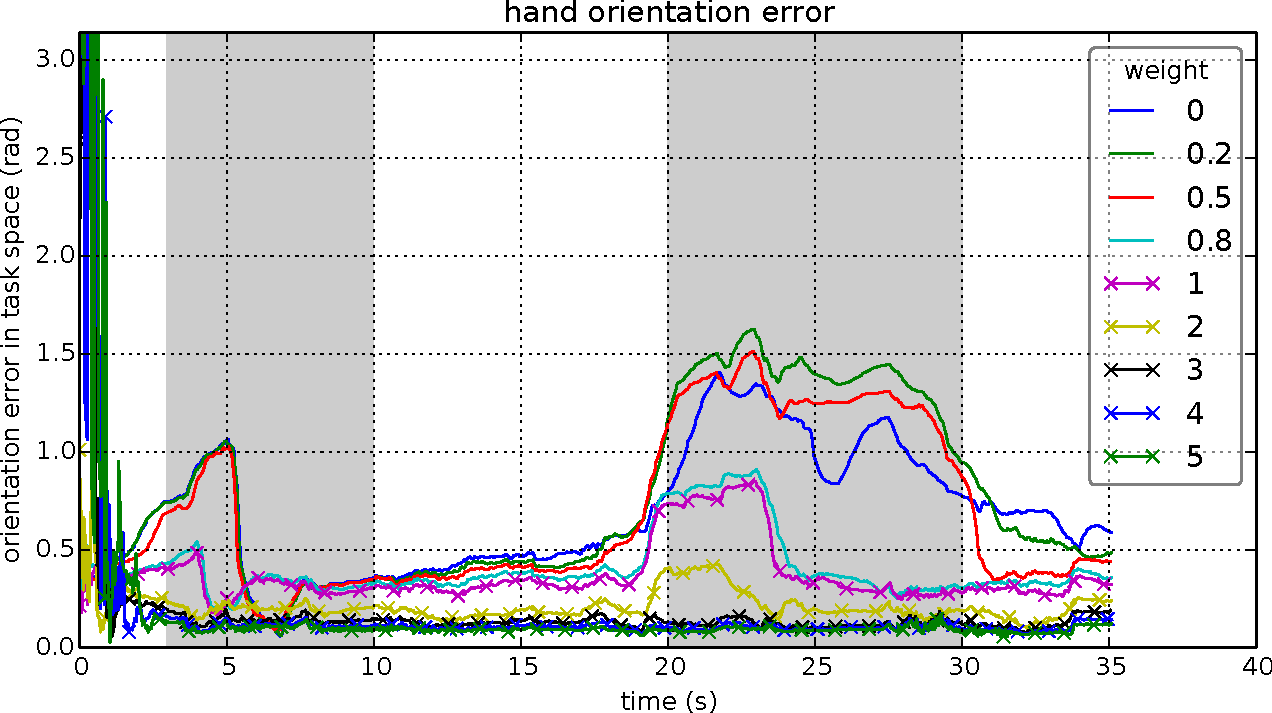
\includegraphics[width=0.5\textwidth]{images/eval_prior/common_weights/stereo_hand_ori_error.pdf}
\label{fig:stereo_hand_ori_error}}
\caption[Task space error (Exp. 1, stereo)]{Task space error for left hand pose (Exp. 1, \textit{stereo} data). (a) The hand position error can already be reduced by minimal weighting of the prior objective. (b) Small weights actually increase the error and higher weights of at least $0.8$ are required to enforce the reported pose.}
\label{fig:stereo_hand_pose_error}
\end{figure}


\paragraph{Asus Xtion}

Using the structured light sensor Asus Xtion, the behaviour of decreasing error with increasing weight is comparable to that seen for the stereo matching sensor. Similar to the stereo sensor (\cref{fig:stereo_joint_error_hand}), the error on the finger joints reduces significantly when using a small weight of $0.2$ (\cref{fig:xtion_joint_error_hand}).
In contrast to the small errors on the arm joints when using stereo in the phase of moving towards the object (\cref{fig:stereo_joint_error_arm}), the error in this phase when using the Xtion sensor is fairly large for no and low weighted prior (\cref{fig:xtion_joint_error_arm}).

\begin{figure}[h]
\centering
\subfloat[finger joints]{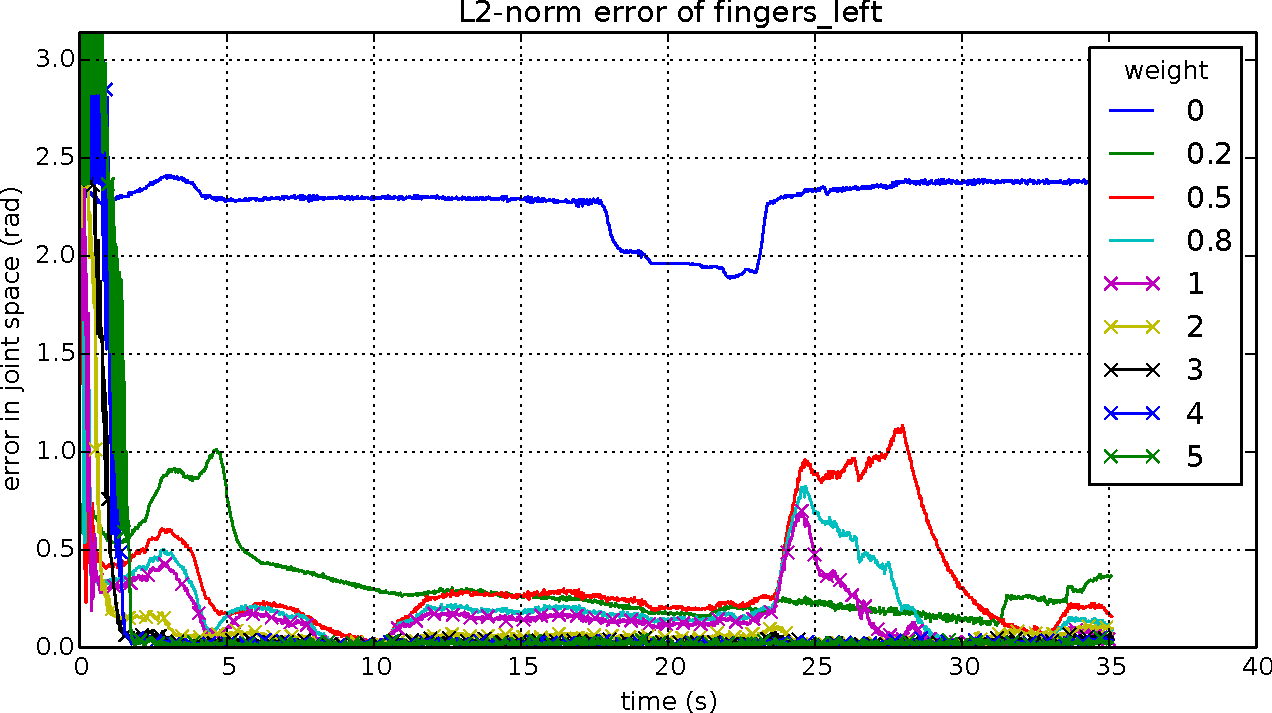
\includegraphics[width=0.5\textwidth]{images/eval_prior/common_weights/xtion_finger_joint_error.pdf} \label{fig:xtion_joint_error_hand}}
%
\subfloat[arm joints]{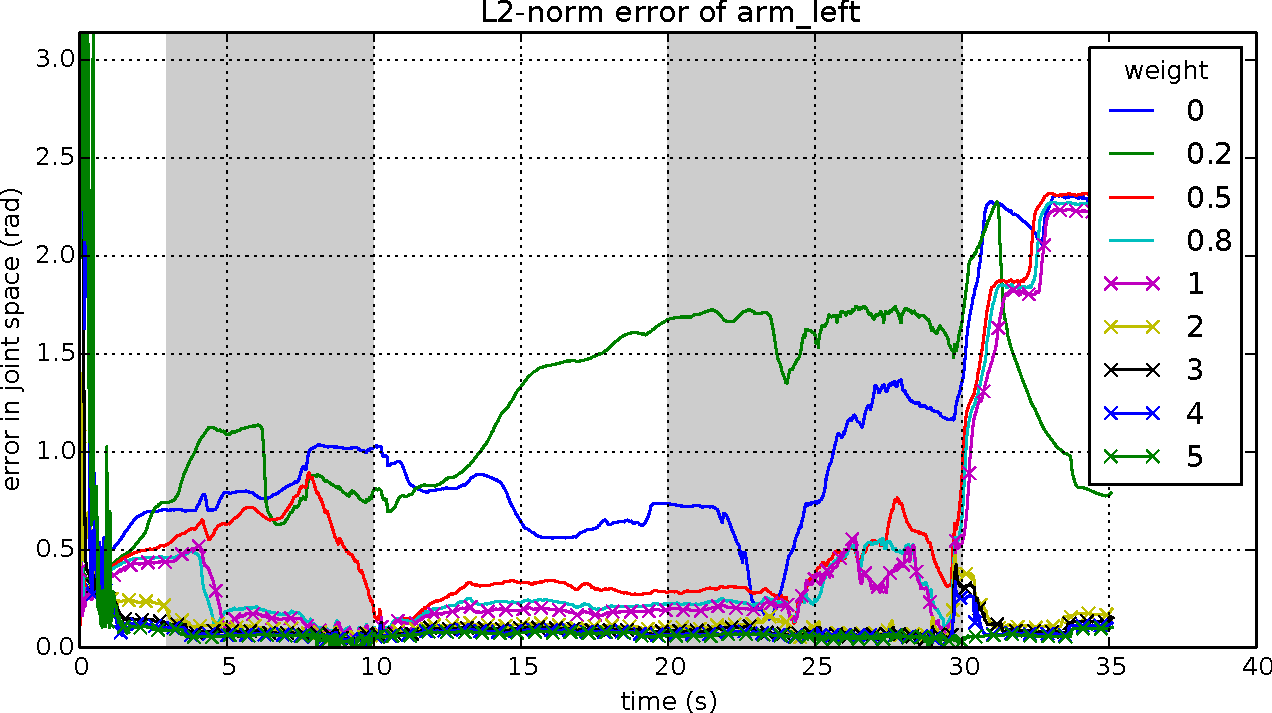
\includegraphics[width=0.5\textwidth]{images/eval_prior/common_weights/xtion_arm_joint_error.pdf} \label{fig:xtion_joint_error_arm}}
\caption[Joint space error (Exp. 1, xtion)]{Joint space error for finger and arm joints (Exp. 1, \textit{xtion} data). Comparable to stereo data set, the finger joint deviation (a) is already reduced by small weights.}
\label{fig:xtion_joint_error}
\end{figure}

As before, the hand pose error is only effected by the arm joint errors and thus the hand position error shown in \cref{fig:xtion_hand_pos_error} is large in the same moving phase close to the object. For using the structured light sensor, a common weight of at least $2$ is required to drive the solution towards the reported hand position.

\begin{figure}[h]
\centering
\subfloat[position error]{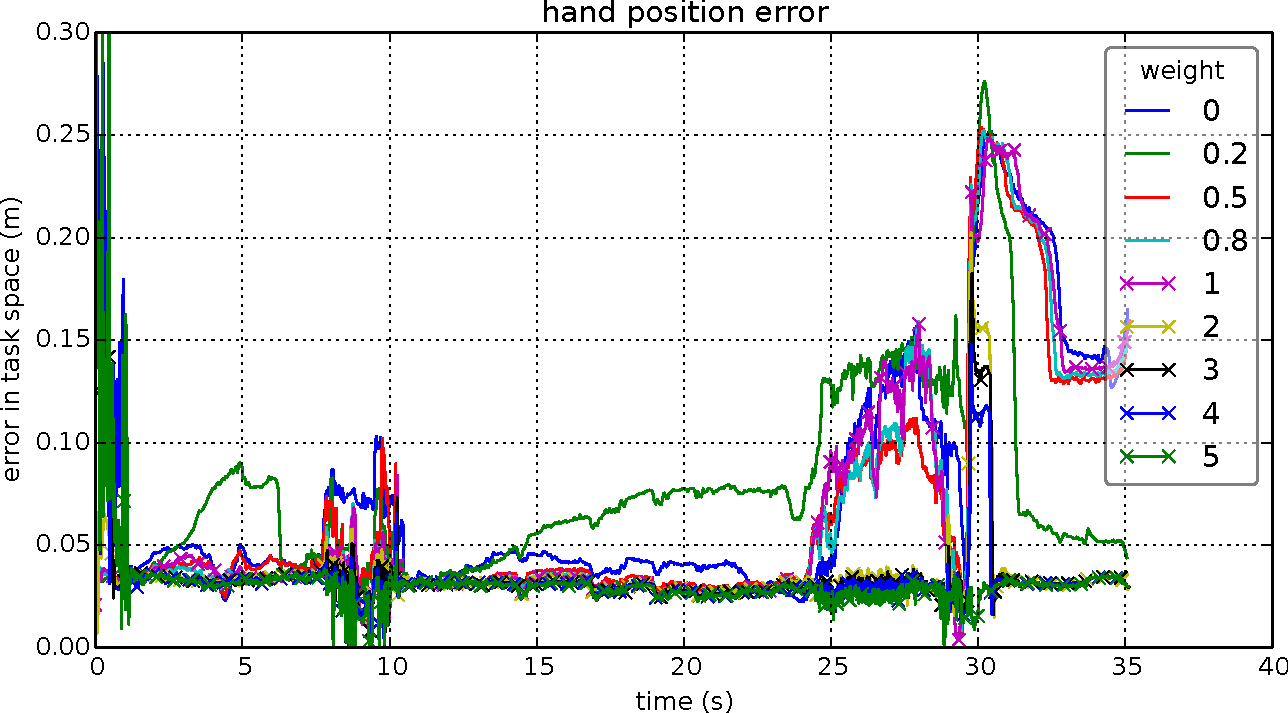
\includegraphics[width=0.5\textwidth]{images/eval_prior/common_weights/xtion_hand_pos_error.pdf} \label{fig:xtion_hand_pos_error}}
%
\subfloat[orientation error]{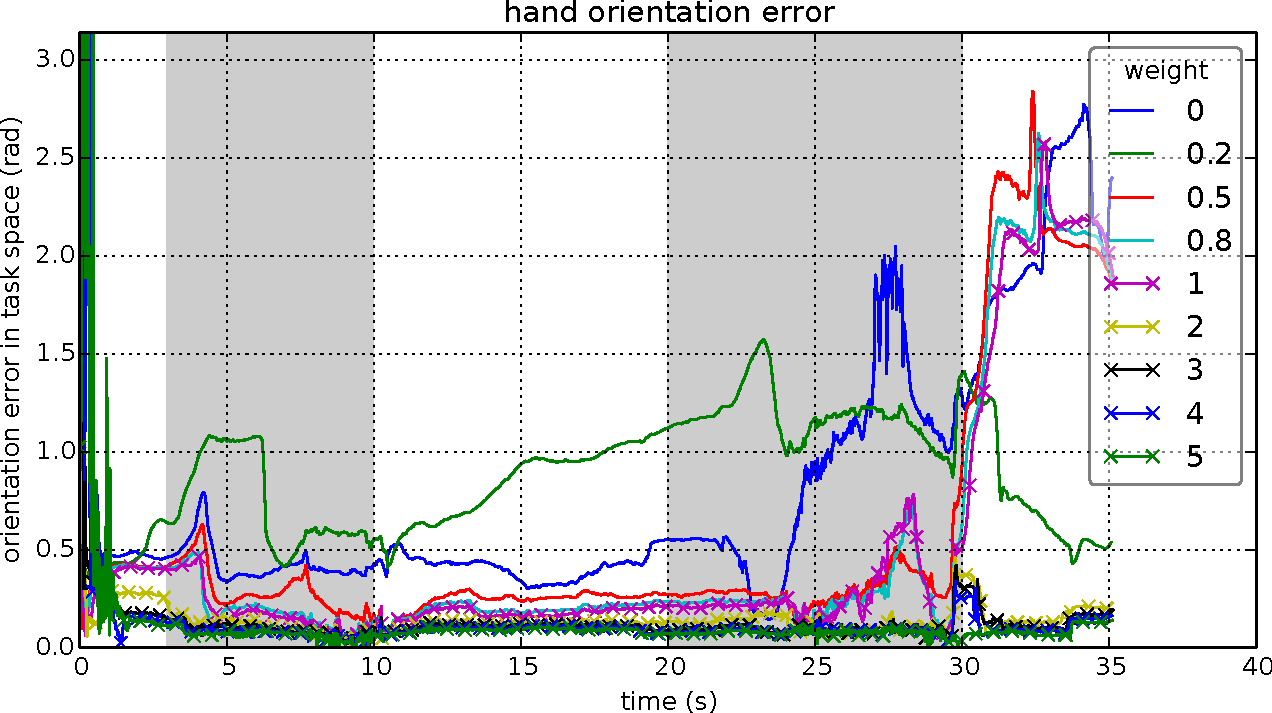
\includegraphics[width=0.5\textwidth]{images/eval_prior/common_weights/xtion_hand_ori_error.pdf} \label{fig:xtion_hand_ori_error}}
\caption[Task space error (Exp. 1, xtion)]{Task space error for left hand pose (Exp. 1, \textit{xtion} data). The pose error this data set has a different characteristic than on the stereo data set. Large weights above $2$ are required to enforce the reported pose.}
\label{fig:xtion_hand_pose_error}
\end{figure}

\subsubsection{Joint Prior Objective with Individual Weights}

Individual weighting is applied to stereo depth data only. This weighting scheme enables us to weight each combination of joint deviations separately as defined by \cref{eqn:objf_indiv_weighted}. For simplicity, only single joint deviations are weighted. That is, the weight matrix $Q$ will be a diagonal matrix where only the diagonal elements $q_{i,i}$ will be defined.

In this scenario, the two palm joints (\texttt{leftWristRoll} and \texttt{leftWristPitch}) that connect the hand with the arm are weighted with increasing weights, while the remaining joints are kept constant at either low weights ($0.2$ for finger joints, $0.2$ for remaining joints) or kept constant at normal weights ($0.2$ for finger joints, $1.0$ for remaining joints).

%In this scenario, three setting of joints are weighted and this scheme is captured in the legend as follows: first, all diagonal elements of $Q$ are set to the weight \emph{q}, second, the 13 finger joints are set to the weight \emph{fingers} and optionally third, the two palm joints (\texttt{leftWristRoll} and \texttt{leftWristPitch}) are set to the value \emph{palm}. E.g., a plot named "\texttt{q 1, fingers 0.2, palm 5}" indicates that finger joints in the diagonal are weighted by $0.2$, palm joints are weighted with $5$ and the remaining joints are weighted with $1$.

%\Cref{fig:indiv_joint_error} shows the joint space error for fingers and arms separately as before.

Because we specifically weight both palm joints, the joint space error of the finger and the arm joints are effected in different ways (\cref{fig:indiv_joint_error}). While the arm joint error reduces with increasing palm weight, the finger joint error actually increases. The reason for this is that both palm joints, as part of the arm kinematic chain, determine the pose of the hand palm. While the hand pose is biased towards the reported pose by the prior, the fingers do not benefit from prior to the same extent.


%From these plots we can see that the individual weighting affects the fingers and the arm in different ways. The finger joint error in \cref{fig:indiv_joint_error_hand} shows that, raising the palm weights and keeping the remaining constant, actually impairs the performance (e.g., compare "\texttt{q 1, fingers 0.2}" with palm weights raised from \texttt{palm 1} to \texttt{palm 5}). In contrast to this, the arm joint error is reduced when increasing the palm weights and keeping remaining weights constant (e.g., compare \texttt{q 0.2, fingers 0.2, palm 5} and palm weights raised to \texttt{q 0.2, fingers 0.2, palm 25}).

\begin{figure}[h]
\centering
\subfloat[finger joints]{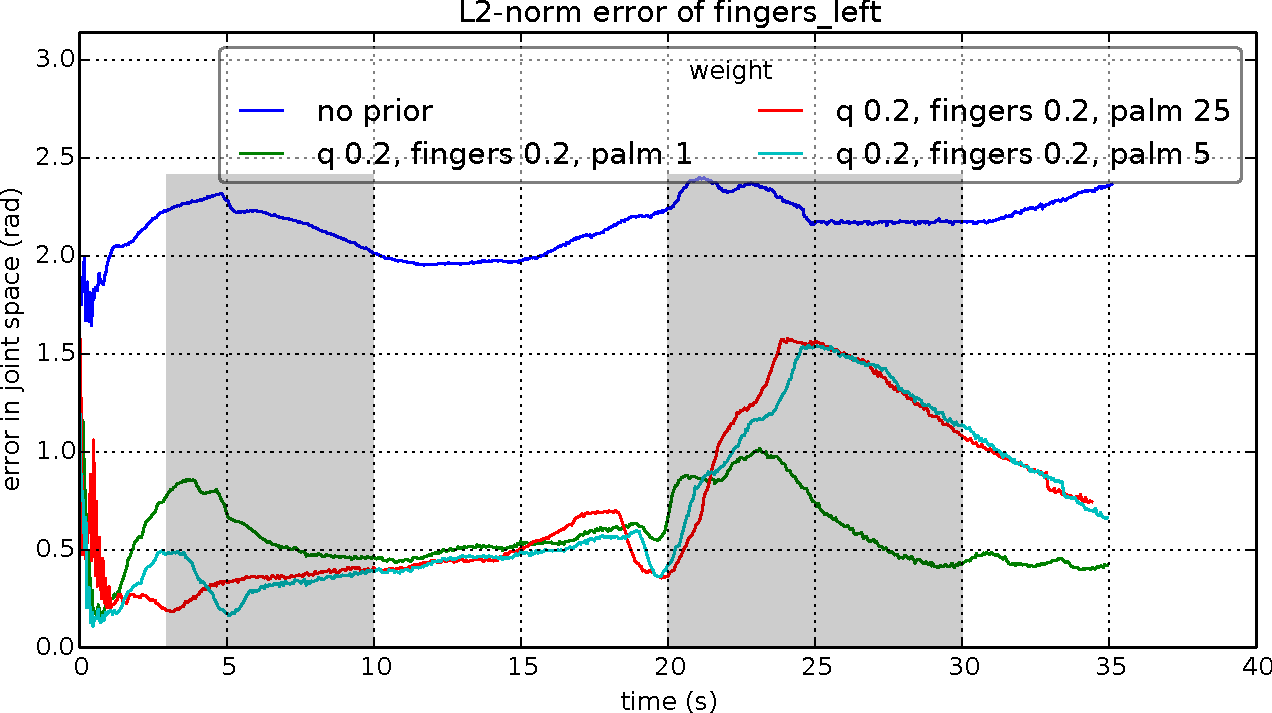
\includegraphics[width=0.5\textwidth]{images/eval_prior/inidv_weights/q0_stereo_finger_joint_error.pdf} }
%
\subfloat[arm joints]{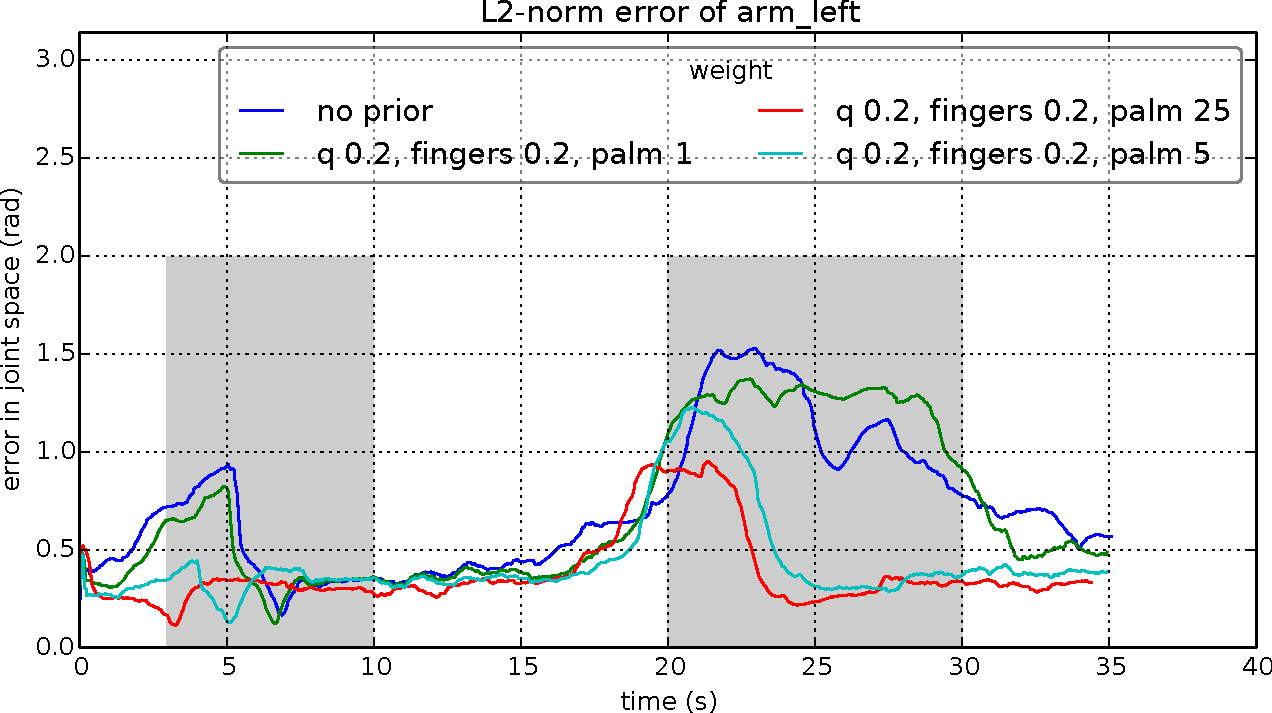
\includegraphics[width=0.5\textwidth]{images/eval_prior/inidv_weights/q0_stereo_arm_joint_error.pdf} }

\subfloat[finger joints]{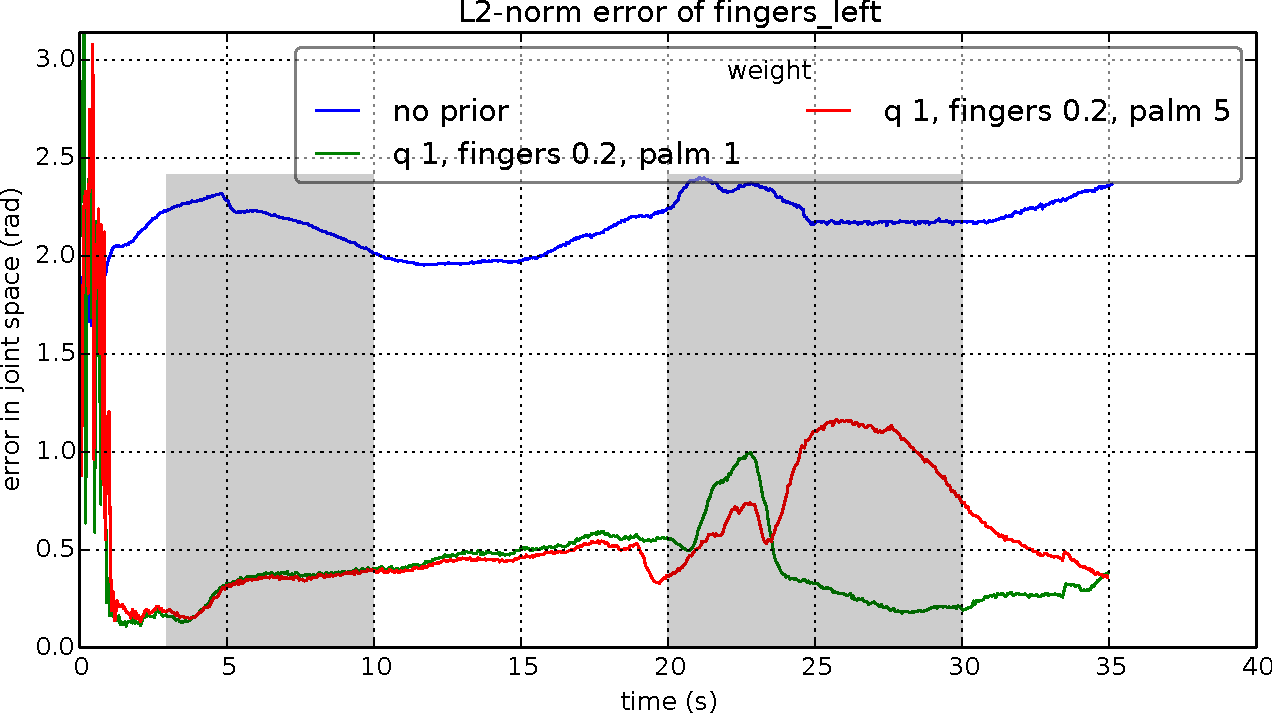
\includegraphics[width=0.5\textwidth]{images/eval_prior/inidv_weights/q1_stereo_finger_joint_error.pdf} }
%
\subfloat[arm joints]{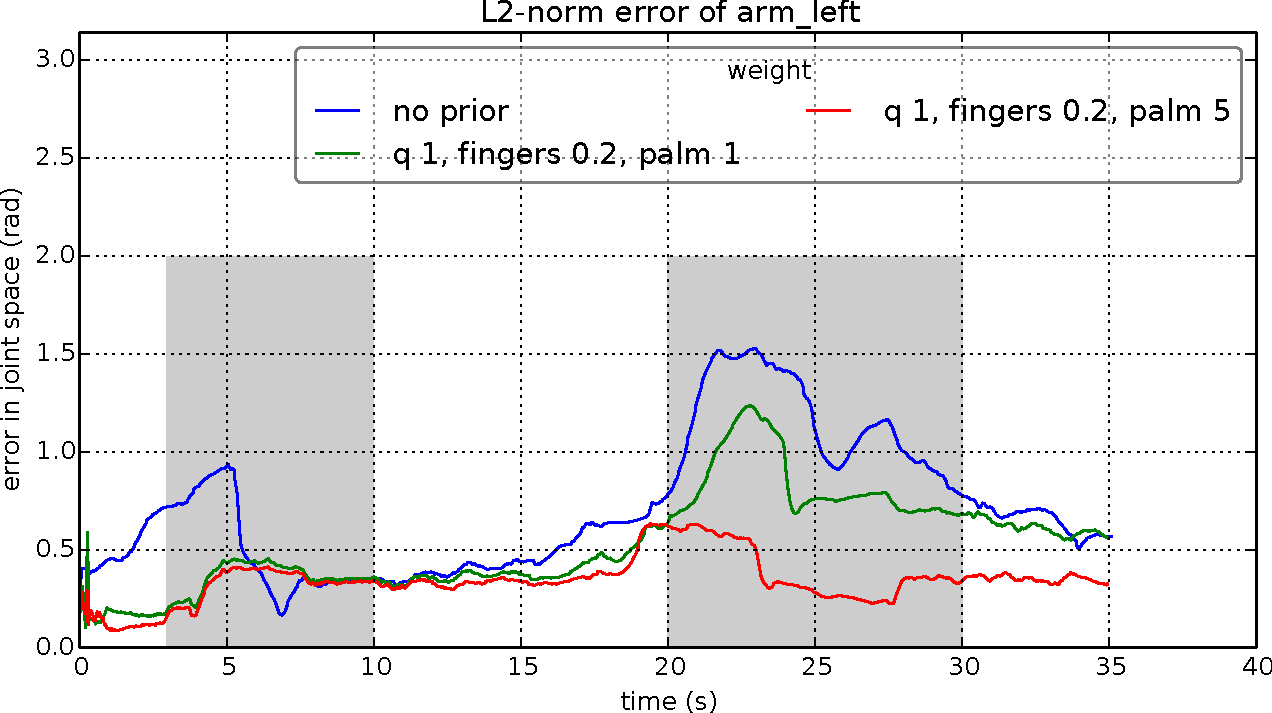
\includegraphics[width=0.5\textwidth]{images/eval_prior/inidv_weights/q1_stereo_arm_joint_error.pdf} }

\caption[Joint space error for individual weighting (Exp. 1)]{Joint space error for individual weighting (Exp. 1). Weights on palm joints are increased ($1$, $5$, $25$) while remaining joints are kept constant at low weights (a,b) or normal weights (c,d). Finger joint errors (a,c) increase with increasing palm weights, while arm joint errors (b,d) are reduced.}
\label{fig:indiv_joint_error}
\end{figure}

%Again, the arm joints directly influence the pose error of the hand as seen in \cref{fig:indiv_pose_error}. \Cref{fig:indiv_hand_pos_error} shows that the hand position mostly benefits from using a weight $>1$ on the palm joints, whereas weighting the remaining joints does not contribute to driving the solution towards the reported hand position. We can also see that using small weights ($q=0.2$) for all joints but the palm actually results in a estimated position closer to the reported position than what is achieved by larger weights ($q=1$).
%For the hand orientation error in \cref{fig:indiv_hand_ori_error}, the error is usually reduced if the weights on the palm joints are increased (e.g. $1$ to $5$, or $5$ to $25$) and remaining joints keep their weights.

The task space error (\cref{fig:indiv_pose_error}) is similarly related to the weight of the palm joints as the arm joint error. By particularly enforcing the reported position on two joints, the hand pose error is reduced while avoiding overshooting effects as seen when applying common weights to all joints.

\begin{figure}
\centering
\subfloat[position error]{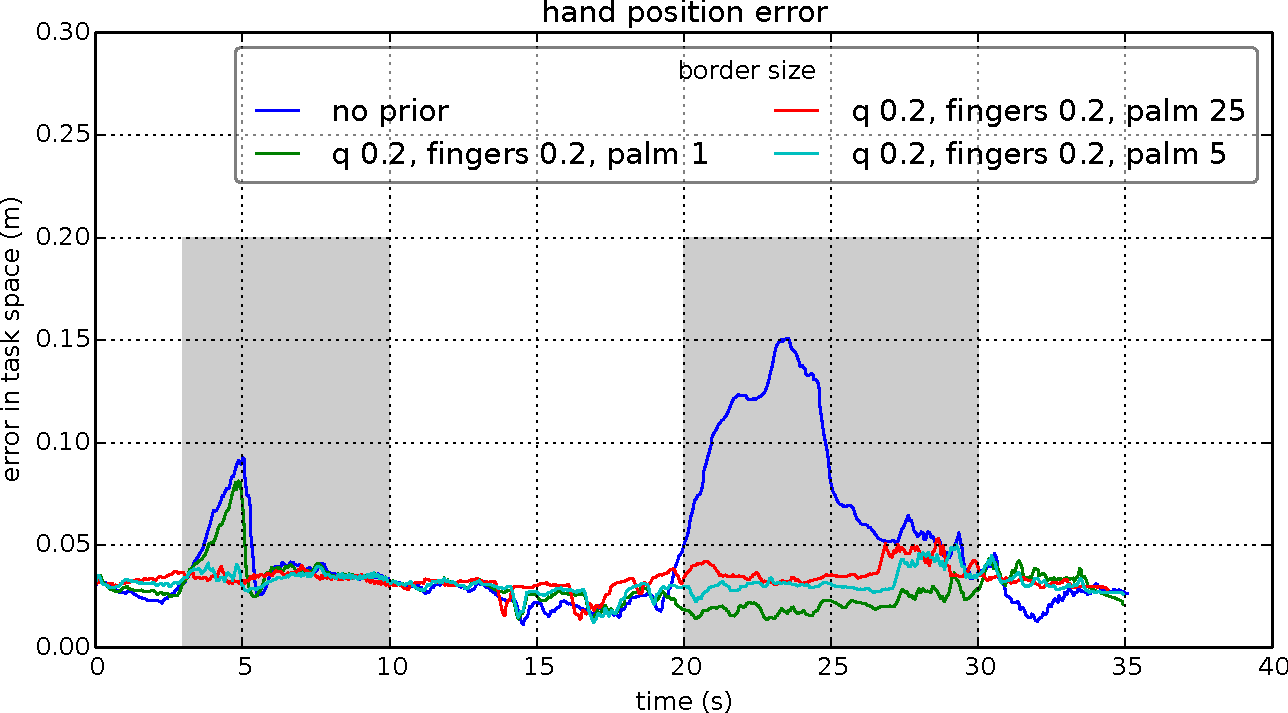
\includegraphics[width=0.5\textwidth]{images/eval_prior/inidv_weights/q0_stereo_hand_pos_error.pdf} }
%
\subfloat[orientation error]{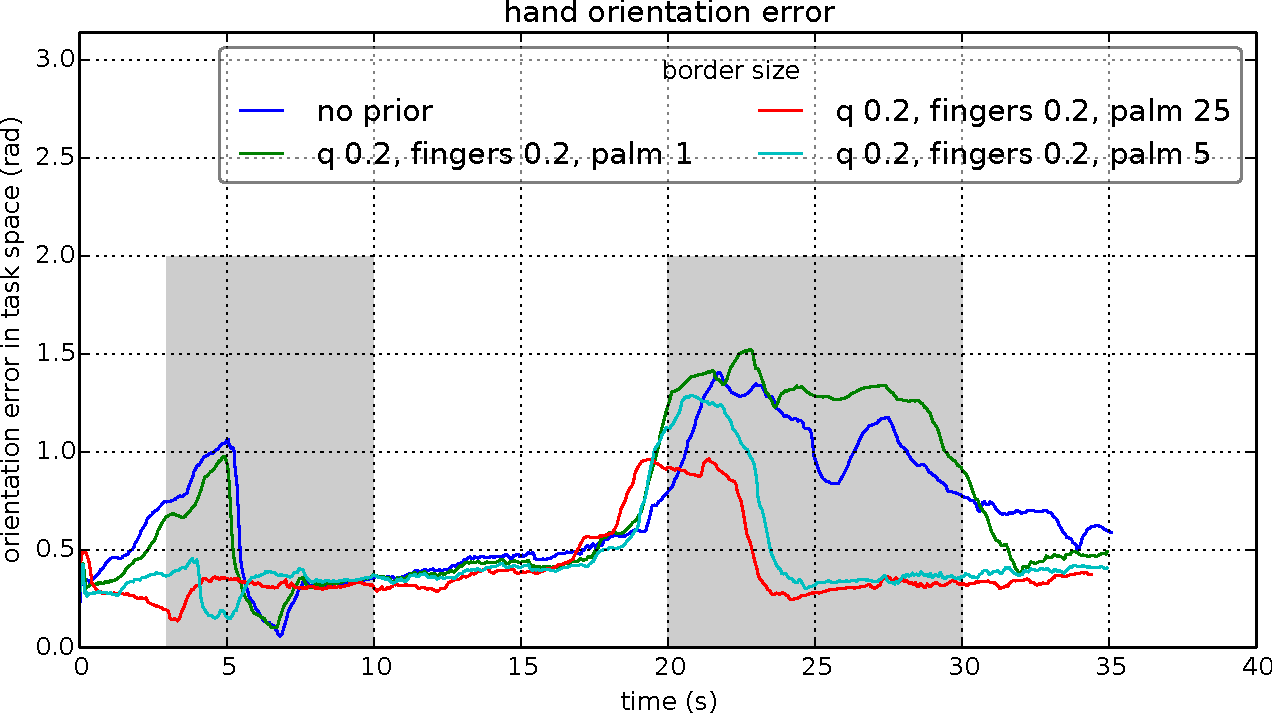
\includegraphics[width=0.5\textwidth]{images/eval_prior/inidv_weights/q0_stereo_hand_ori_error.pdf} }

\subfloat[position error]{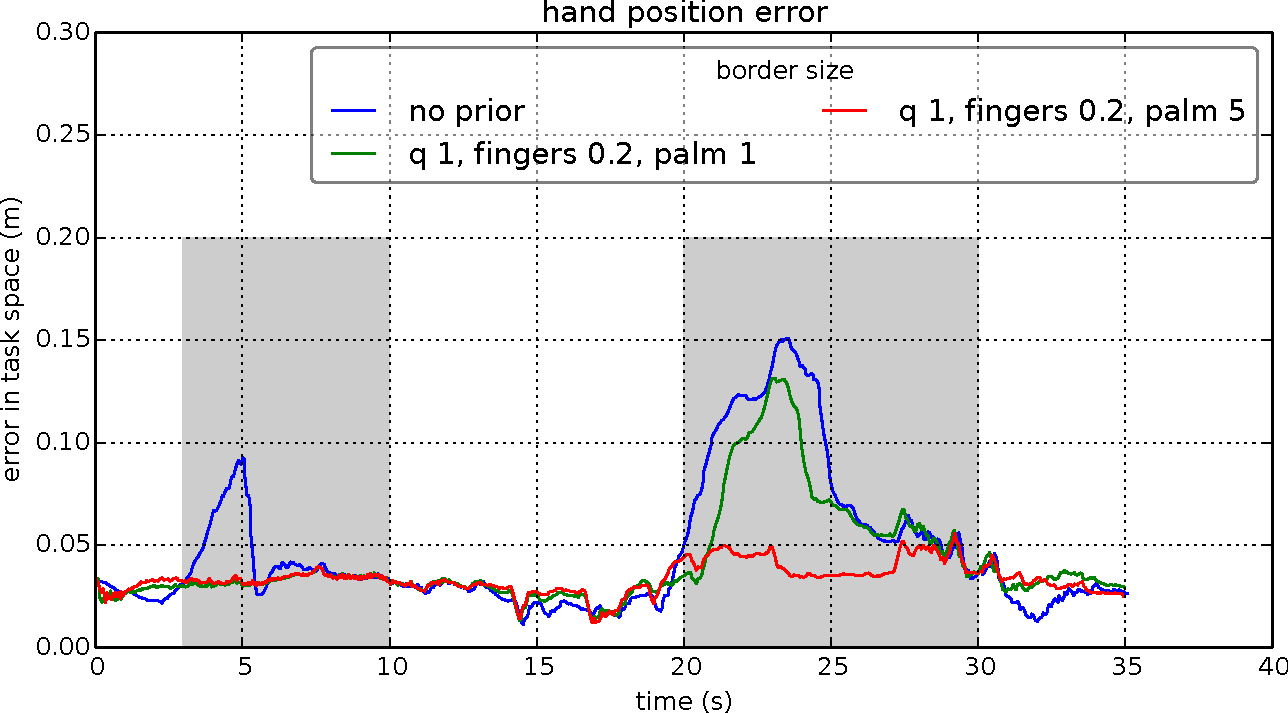
\includegraphics[width=0.5\textwidth]{images/eval_prior/inidv_weights/q1_stereo_hand_pos_error.pdf} }
%
\subfloat[orientation error]{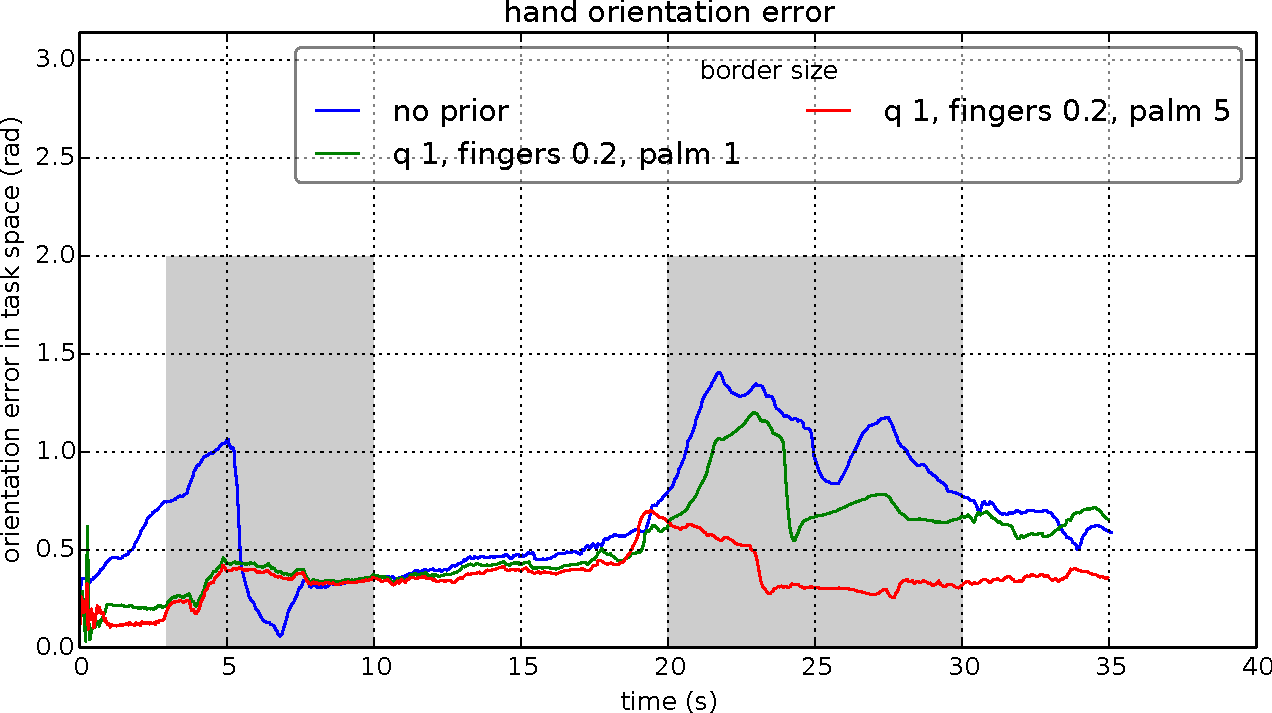
\includegraphics[width=0.5\textwidth]{images/eval_prior/inidv_weights/q1_stereo_hand_ori_error.pdf} }

\caption[Task space error for individual weighting (Exp. 1)]{Task space error for individual weighting (Exp. 1). Weights on palm joints are increased ($1$, $5$, $25$) while remaining joints are kept constant at low weights (a,b) or normal weights (c,d). The hand pose error is reduced in each case for increasing palm weights.}
\label{fig:indiv_pose_error}
\end{figure}

%\subsubsection{Object Position}
%
%Most of the time, the pose of the object (bottle) is mainly affected by the optimization. Only when there is interaction between the manipulator and the object, it gets indirectly dependant on the joint values and hence the prior weight. The object's pose is manually initialised close to the true observed state and is expected to not move until the end of the reaching phase. \Cref{fig:bottle_movement} compares the object's distance to the image origin for stereo and xtion data sets and gives an indication about its movement. The bottle in the stereo data (\cref{fig:bottle_movement_stereo}) stays, as expected, close to its initial position until the end of the reaching phase. In contrast, the bottle in the Xtion data set (\cref{fig:bottle_movement_xtion}) already moves at the beginning to its final pose.
%
%\begin{figure}[h]
%\centering
%\subfloat[stereo]{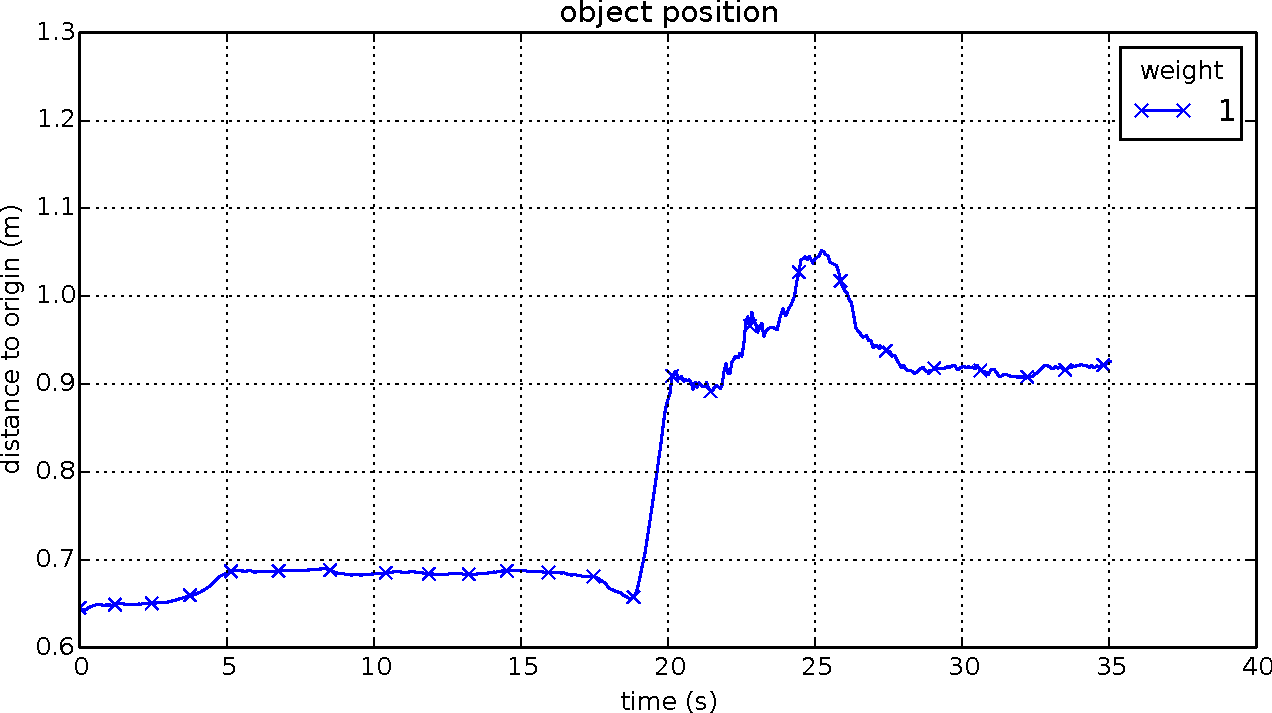
\includegraphics[width=0.5\textwidth]{images/eval_prior/stereo_obj_pos.pdf} \label{fig:bottle_movement_stereo}}
%\subfloat[xtion]{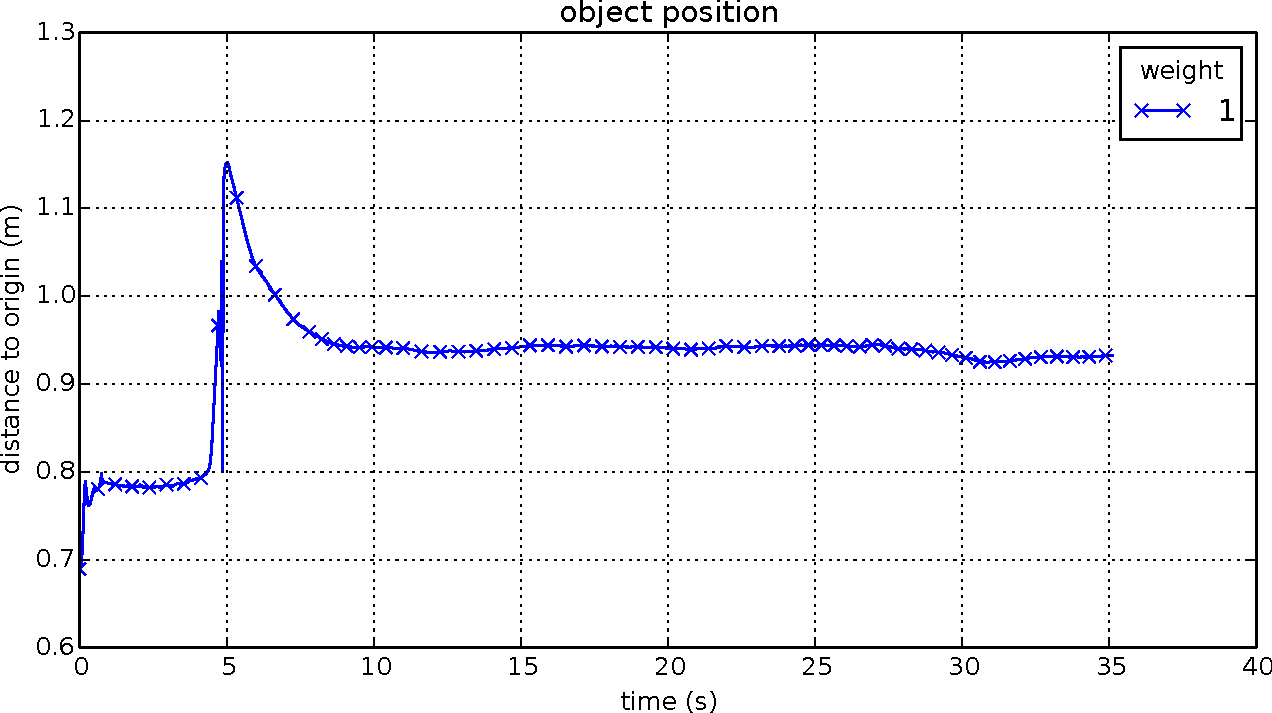
\includegraphics[width=0.5\textwidth]{images/eval_prior/xtion_obj_pos.pdf} \label{fig:bottle_movement_xtion}}
%\caption{Movement of bottle during robot arm movement}
%\label{fig:bottle_movement}
%\end{figure}
%
%Snapshots of the perceived point clouds are depicted in \cref{fig:bottle_point_cloud} for a state at the beginning of the experiment for both depth sources. A comparison of these sources show that: 1) the stereo depth source contains data with larger depth, and 2) the stereo depth source also contains more points of the object than the structured light sensor. It must be noted that the structured light sensor is mounted above the stereo sensor pointing into the same region of interest. It thus perceives the scene at a steeper angle.
%
%\begin{figure}
%\centering
%\subfloat[stereo point cloud]{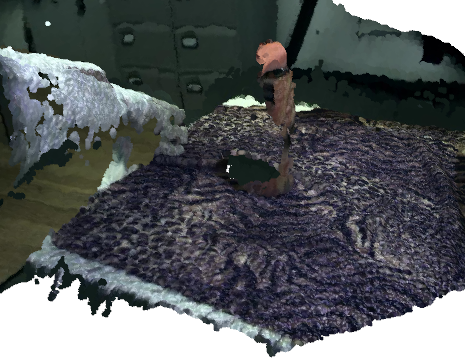
\includegraphics[width=0.4\textwidth]{images/eval_prior/stereo_bottle.png} }
%\hspace{1cm}
%\subfloat[xtion point cloud]{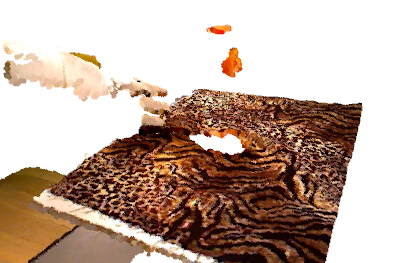
\includegraphics[width=0.4\textwidth]{images/eval_prior/xtion_bottle.png} }
%\caption{Table and bottle in stereo and xtion point cloud}
%\label{fig:bottle_point_cloud}
%\end{figure}


\subsubsection{Self-Observation Filtering using Joint Prior}

An alternative to using prior information in the optimization is to use prior information to provide the optimization with relevant data. In this sense, the reported state of the robot is used to filter its observation to only contain points close to the predicted location of the manipulator.
%In this scenario, the object is not included in tracking as relevant points cannot be obtained by self-observation.

The filtering of observed data is achieved by projecting the manipulator into the field-of-view of the robot's perception system. Each point in the disparity image that is occupied by one of the robot's projected parts is kept while all remaining values are removed. This filtered region can be further expanded on the borders of the self perceived parts. \Cref{fig:self_observation_region} demonstrates the filtered perception on stereo data for three different values for the border expansion.
%The expansion value is the size of the squared dilation kernel that is applied to the self-observation mask.

\begin{figure}[h]
\centering
\subfloat[normal mask]{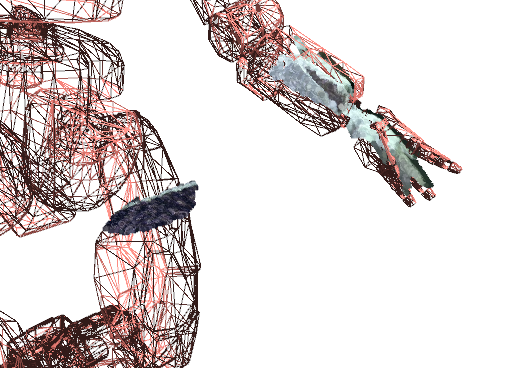
\includegraphics[width=0.3\textwidth]{images/eval_prior/filtering/filt_b0.png} }
\subfloat[expanded by 10 pxl]{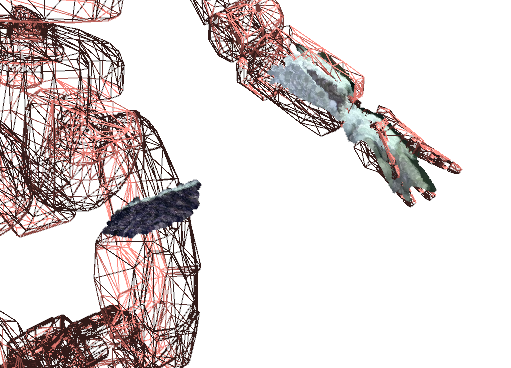
\includegraphics[width=0.3\textwidth]{images/eval_prior/filtering/filt_b10.png} }
\subfloat[expanded by 100 pxl]{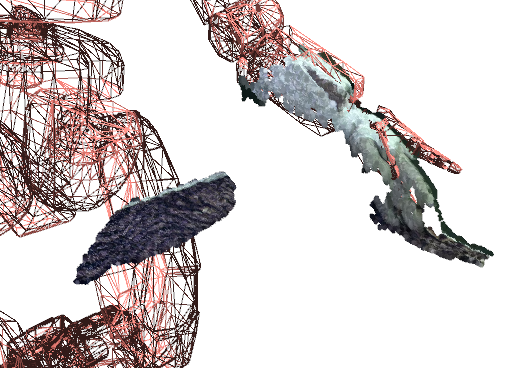
\includegraphics[width=0.3\textwidth]{images/eval_prior/filtering/filt_b100.png} }
\caption[Self-Observation filtering]{Point cloud filtering by self-observation with different expended regions.}
\label{fig:self_observation_region}
\end{figure}

In comparison to the joint position prior applied to the objective function, the joint and task space errors for self-observation filtering are given in \cref{fig:filter_joint_error,fig:filter_pose_error}. The error is again given as the deviation from the reported pose, however the joint position prior is not used in the optimization and hence, the solution is not directly driven towards the reported configuration.

As it can be easily seen for the joint space error in \cref{fig:filter_joint_error_hand,fig:filter_joint_error_arm}, there is an individual optimal value for the region expanding that minimizes the error for the finger joints (20) and the arm joints (150). While the finger joint deviation in the optimal expanded case is larger than the joint deviation using small weights (\cref{fig:stereo_joint_error_hand}), the optimal arm region expansion achieves similar results compared to the joint prior with weights around $1$ (\cref{fig:stereo_joint_error_arm}).

\begin{figure}[h]
\centering
\subfloat[finger joints]{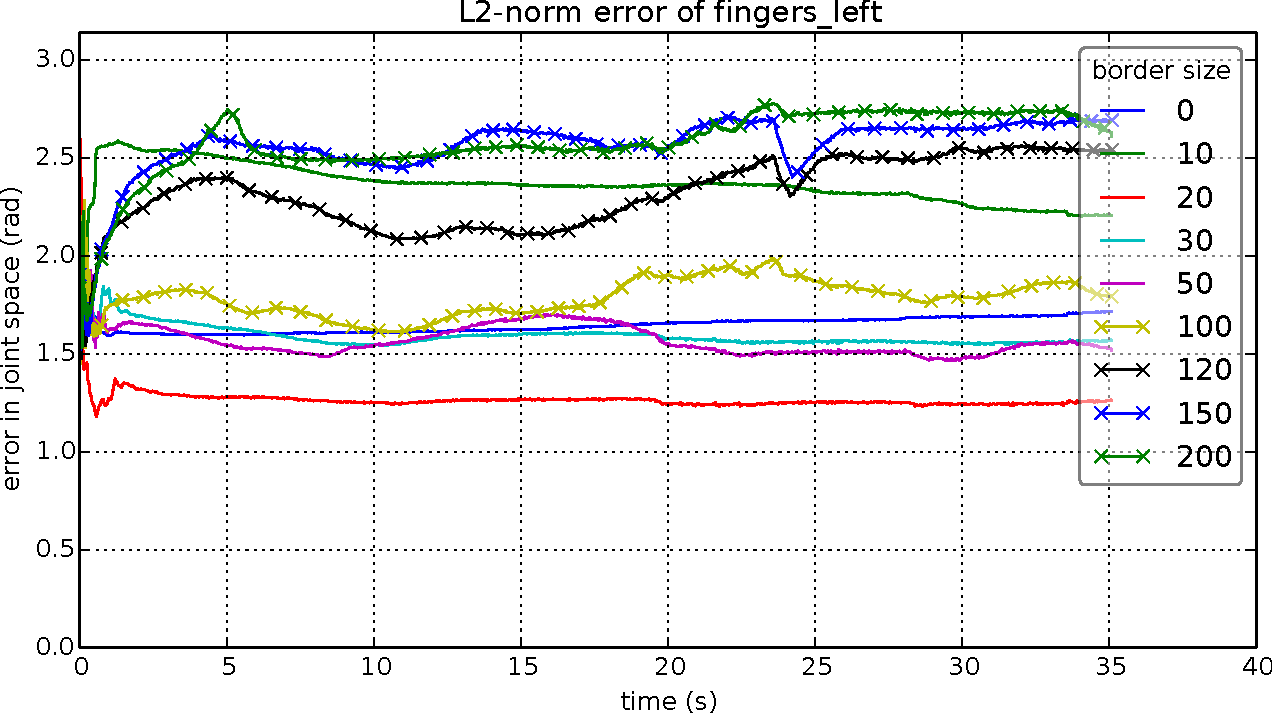
\includegraphics[width=0.5\textwidth]{images/eval_prior/filtering/stereo_finger_joint_error.pdf} \label{fig:filter_joint_error_hand}}
\subfloat[arm joints]{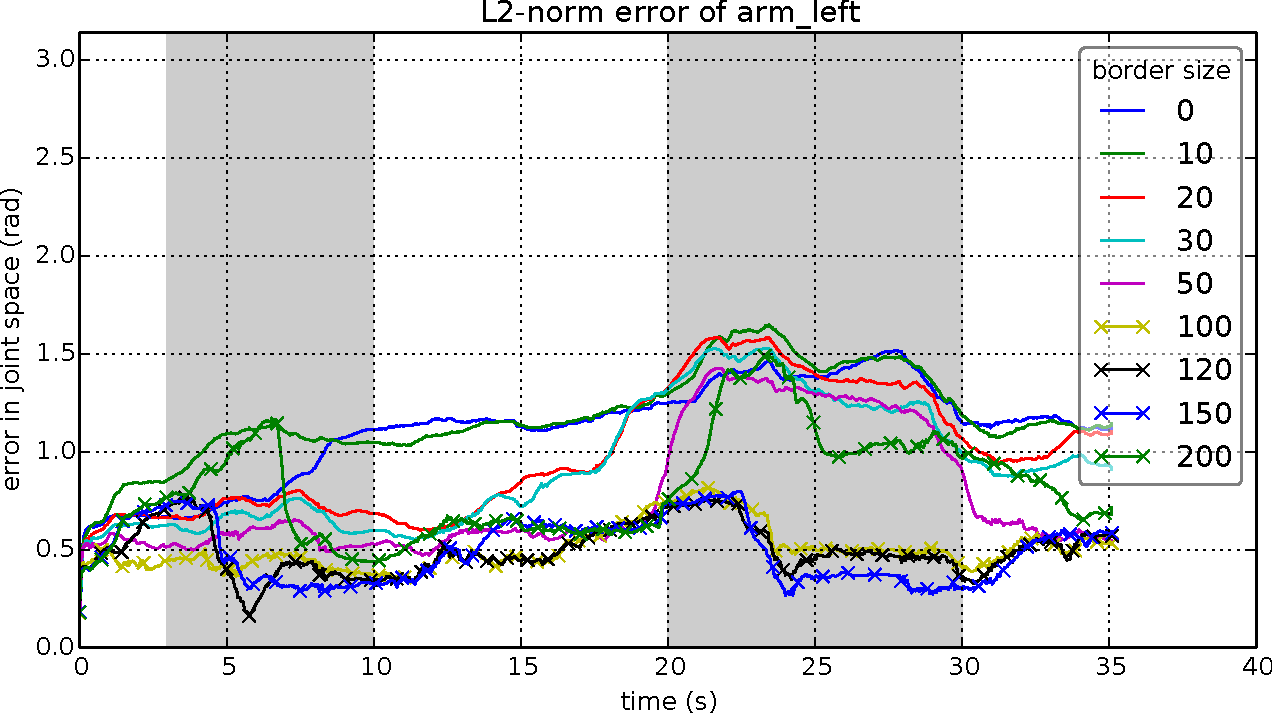
\includegraphics[width=0.5\textwidth]{images/eval_prior/filtering/stereo_arm_joint_error.pdf} \label{fig:filter_joint_error_arm}}
\caption{Joint space error for filtered perception (Exp. 1)}
\label{fig:filter_joint_error}
\end{figure}

For large expansions of the self-observation mask (200), the hand position error in \cref{fig:filter_hand_pos_error} behaves similar to the case where no prior is used on the unfiltered observation (\cref{fig:stereo_hand_pos_error}). Further, in phases of contact with surrounding objects a smaller region expansion is preferable over larger borders. The reason for this is that large self-observation masks will include nearby objects, which again will distract the optimization without prior. A larger region expansion is preferable in phases where the manipulator is moving in free space (time between highlighted phases).
The hand orientation error behaves similar to the arm joint error, in particular an optimal region expansion (150) emerges and larger region expansions are favourable in general.

\begin{figure}
\centering
\subfloat[position error]{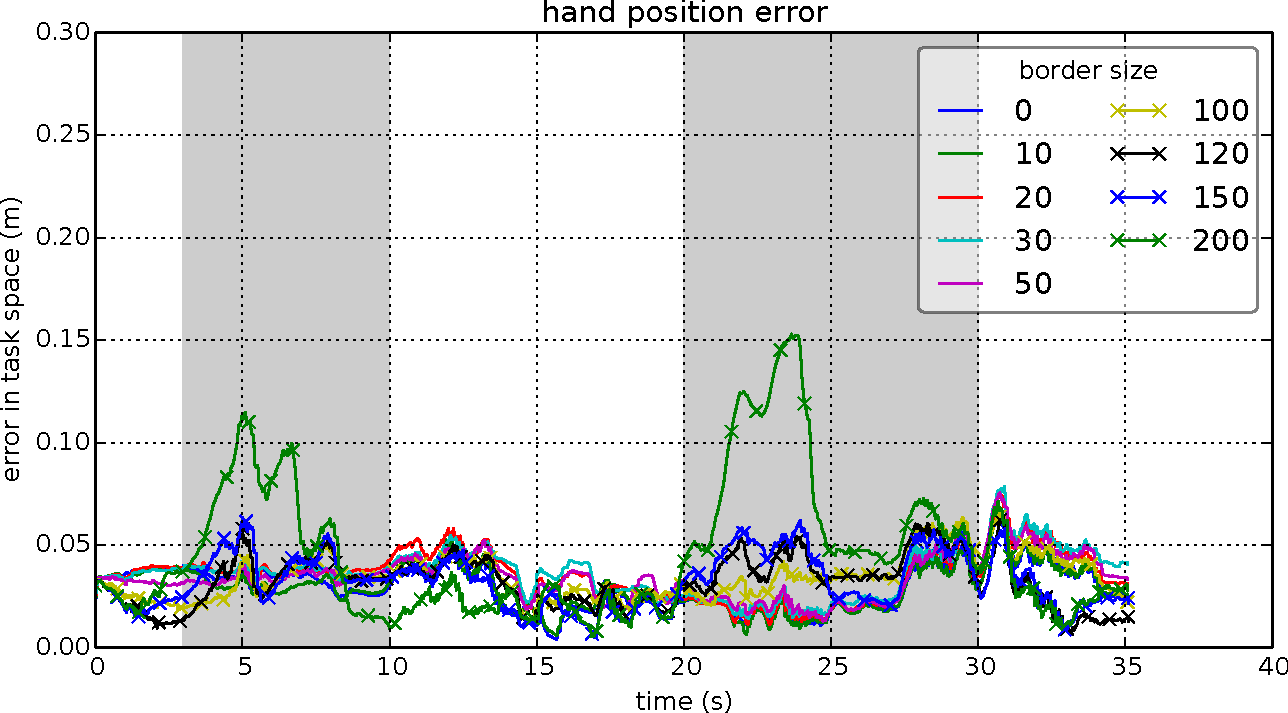
\includegraphics[width=0.5\textwidth]{images/eval_prior/filtering/stereo_hand_pos_error.pdf} \label{fig:filter_hand_pos_error}}
\subfloat[orientation error]{\includegraphics[width=0.5\textwidth]{images/eval_prior/filtering/stereo_hand_ori_error.pdf} \label{fig:filter_hand_ori_error}}
\caption{Task space error for filtered perception (Exp. 1)}
\label{fig:filter_pose_error}
\end{figure}


\subsection{Interpretation}

With the signed distance as the only objective function, the optimization is driven away from the reported state, with which it is initialized, whenever nearby but unrelated depth data is assigned to the robot model. Hence we conclude that \cref{hyp:distracting_readings} is true. By augmenting the objective function with an objective related to the reported state as the reference, this effect can be reduced.

Across all weighting schemes and depth sources, we can see that weighting in respect to the deviation from the reported pose: (1) reduces the deviation of finger joint positions over the whole sequence of the trials by already choosing a small prior weight, (2) contributes most in movement phases that follow states where the manipulator is in contact with the scene (table, object). The application of individual weighting of joint deviations showed that by selecting specific joints, the task space error can be reduced while keeping the flexibility of preferring other objectives for the remaining parts of the robot model. For both assessed weighting schemes, it turned out that weights need to be chosen carefully to prevent overshooting on the reported state and hence the oscillation of the estimate state. Neglecting the issue of oscillating around the optimum, \cref{hyp:prior_information} is also considered to be verified.

The self-observation filtering of the perception showed that using prior information to shape the input to the optimization also counteracts the issue of distracting observation. By using prior information to filter relevant data, the reported robot state only indirectly improves the optimization result.
The decoupling of the optimization from the reported joint values prevents cases of overfitting on the reported state by limiting the bias from prior information.

The assessed prior information is by design only applicable to the robot model. The tracked object remains to be driven by the signed distance function and hence relies on relevant depth data assigned to the object model. We saw that this is an issue for observing from an low angle to the object's principal axes.


\section{Experiment 2: Ground Truth Comparison}
\label{sec:hand_pose_error}

An experiment was conducted that contains depth data measurements from the manipulator alone, without distracting depth readings nearby. As in the previous experiment, forward kinematics on the reported and estimated joint configuration was used to obtain the pose of the manipulator in task space. Additionally, the Vicon system introduced earlier provides ground truth data of the hand palm pose.


\subsection{Hypotheses}

The experiment has been designed to (1) apply the tracking of the manipulator in a scene without distractions, and (2) to compare the reported and estimated robot configuration with the ground truth poses reported by the Vicon tracking system.

Without distracting sensor readings, we expect that the use of the joint position prior will not have a strong impact on the deviation from the reported robot configuration. If the manipulator is fully observed in the depth data, tracking the manipulator should result in a hand pose close to the true hand pose which itself should coincide with the reported hand pose.

\begin{hypothesis}(No effect of joint position prior)\\
There is no significant effect of applying a joint position prior on observations containing solely the manipulator.
\label{hyp:no_prior_effect}
\end{hypothesis}

\begin{hypothesis}(Matching hand pose)\\
Reported and estimated left hand poses agree with the measured hand pose.
\label{hyp:matching_hand_pose}
\end{hypothesis}


\subsection{Setup}

The robot is placed in a nominal position and its manipulator moves from this state into the field of view of the camera (\cref{fig:vicon_free_movement}). To observe the manipulator and its fingers from different perspectives, the hand and the fingers are actuated by a certain degree. The data set is therefore divided into two parts: \textit{arm movement} (experiment 2a), where mainly the shoulder and the forearm joints are actuated, and \textit{finger movement} (experiment 2b) where all fingers are actuated at the same time. During the complete experiment, Vicon markers are attached to the pelvis and backside of the palm to track the orientation of both robot frames (\cref{fig:vicon_marker}).

\begin{figure}[h]
\captionsetup{width=0.4\textwidth}
\centering
\includegraphics[width=0.4\textwidth]{images/eval_vicon/sequence/setting.png}
\caption[Experiment 2: Setup]{Experiment 2: Setup in which a robot is observing its own manipulator.}
\label{fig:vicon_free_movement}
\end{figure}

\paragraph{Experiment 2a:}
The \textit{arm movement} sequence contains three phases (\cref{tab:vic_arm_movement_phases}) of which 3 final states are depicted in \cref{fig:arm_movement_states}.

\begin{table}[h]
\centering
\begin{tabular}{|c|l|l|}
\hline
 & \emph{time (s)} & \emph{movement description} \\
\hline
1 & 0$\dots$50 & no movement, hand in lower camera view \\
\hline
2 & 50$\dots$54 & arm movement up \\
\hline
3 & 85$\dots$90 & hand palm turning up (forearm joint) \\
\hline
4 & 125$\dots$130 & hand palm turning down (forearm joint) \\
\hline
\end{tabular}
\caption{Phases of arm movement (Exp. 2a)}
\label{tab:vic_arm_movement_phases}
\end{table}

\newlength{\imgwidth}
\setlength{\imgwidth}{0.26\textwidth}

\begin{figure}
\centering
\begin{tabular}{cc:c:c}
& \textit{Phase 2 (t=55\si{\second})} & \textit{Phase 3 (t=91\si{\second})} & \textit{Phase 4 (t=132\si{\second})} \\
& (facing towards robot) & (facing up) & (facing down)\\
\rotatebox{90}{ \hspace{0.8cm} camera image } & \includegraphics[width=\imgwidth]{images/eval_vicon/sequence/arm_movement/arm_movement_cam_view55.png} & \includegraphics[width=\imgwidth]{images/eval_vicon/sequence/arm_movement/arm_movement_cam_view91.png} & \includegraphics[width=\imgwidth]{images/eval_vicon/sequence/arm_movement/arm_movement_cam_view132.png} \\
\rotatebox{90}{ \hspace{1cm} point cloud } & \includegraphics[width=\imgwidth]{images/eval_vicon/sequence/arm_movement/obs_55.png} & \includegraphics[width=\imgwidth]{images/eval_vicon/sequence/arm_movement/obs_91.png} & \includegraphics[width=\imgwidth]{images/eval_vicon/sequence/arm_movement/obs_132.png} \\
\rotatebox{90}{ \hspace{1cm} reported state } & \includegraphics[width=\imgwidth]{images/eval_vicon/sequence/arm_movement/rep_55.png} & \includegraphics[width=\imgwidth]{images/eval_vicon/sequence/arm_movement/rep_91.png} & \includegraphics[width=\imgwidth]{images/eval_vicon/sequence/arm_movement/rep_132.png} \\
\end{tabular}
\caption[Arm movement sequence]{Experiment 2a (\textit{arm movement}): Sequence of states in which the manipulator is observed from different viewing angles. \textit{Upper row:} camera image, \textit{Middle row:} point cloud observation, \textit{Lower row:} reported state.}
\label{fig:arm_movement_states}
\end{figure}

\FloatBarrier

\paragraph{Experiment 2b:}
The \textit{finger movement} sequence contains 7 phases in total (\cref{tab:vic_finger_movement_phases}) of which 6 states are depicted in \cref{fig:finger_movement_states}. Both sequences show that due to self-occlusion, the manipulator cannot be fully observed in a single time instance. In states where the palm is facing down, the Vicon marker can be observed in the point cloud data.

\begin{table}[h]
\centering
\begin{tabular}{|c|l|l|}
\hline
 & \emph{time (s)} & \emph{movement description} \\
\hline
1 & 0$\dots$30 & no movement, palm facing towards camera \\
\hline
2 & 30$\dots$33 & fingers closing 25\% \\
\hline
3 & 56$\dots$59 & fingers closing 50\% \\
\hline
4 & 72$\dots$75 & fingers opening \\
\hline
5 & 100$\dots$104 & hand palm turning up (forearm joint) \\
\hline
6 & 127$\dots$130 & fingers closing 25\% \\
\hline
7 & 147$\dots$150 & fingers closing 50\% \\
\hline
8 & 156$\dots$159 & fingers opening \\
\hline
\end{tabular}
\caption{Phases of finger movement (Exp. 2b)}
\label{tab:vic_finger_movement_phases}
\end{table}

%\newlength{\imgwidth}
\setlength{\imgwidth}{0.26\textwidth}

\begin{figure}
\centering
\begin{tabular}{cc:c:c}
\hline
& \textit{Phase 1 (t=19\si{\second})} & \textit{Phase 2 (t=33\si{\second})} & \textit{Phase 3 (t=61\si{\second})}\\
& (opened) & (closed $\sim 25\%$) & (closed $\sim 50\%$)\\

\rotatebox{90}{ \hspace{0.25cm} camera image } & \includegraphics[width=\imgwidth]{images/eval_vicon/sequence/finger_movement/finger_movement_cam_view19.png} & \includegraphics[width=\imgwidth]{images/eval_vicon/sequence/finger_movement/finger_movement_cam_view33.png} & \includegraphics[width=\imgwidth]{images/eval_vicon/sequence/finger_movement/finger_movement_cam_view61.png} \\

\rotatebox{90}{ \hspace{0.25cm} point cloud } & \includegraphics[width=\imgwidth]{images/eval_vicon/sequence/finger_movement/obs_0.png} & \includegraphics[width=\imgwidth]{images/eval_vicon/sequence/finger_movement/obs_33.png} & \includegraphics[width=\imgwidth]{images/eval_vicon/sequence/finger_movement/obs_61.png} \\

\rotatebox{90}{ \hspace{0.25cm} reported state } & \includegraphics[width=\imgwidth]{images/eval_vicon/sequence/finger_movement/rep_0.png} & \includegraphics[width=\imgwidth]{images/eval_vicon/sequence/finger_movement/rep_33.png} & \includegraphics[width=\imgwidth]{images/eval_vicon/sequence/finger_movement/rep_61.png} \\
\hline
& \textit{Phase 5 (t=105\si{\second})} & \textit{Phase 6 (t=133\si{\second})} & \textit{Phase 7 (t=152\si{\second})}\\
& (opened) & (closed $\sim 25\%$) & (closed $\sim 50\%$)\\

\rotatebox{90}{ \hspace{0.25cm} camera image } & \includegraphics[width=\imgwidth]{images/eval_vicon/sequence/finger_movement/finger_movement_cam_view105.png} & \includegraphics[width=\imgwidth]{images/eval_vicon/sequence/finger_movement/finger_movement_cam_view133.png} & \includegraphics[width=\imgwidth]{images/eval_vicon/sequence/finger_movement/finger_movement_cam_view152.png} \\

\rotatebox{90}{ \hspace{0.25cm} point cloud } & \includegraphics[width=\imgwidth]{images/eval_vicon/sequence/finger_movement/obs_105.png} & \includegraphics[width=\imgwidth]{images/eval_vicon/sequence/finger_movement/obs_133.png} & \includegraphics[width=\imgwidth]{images/eval_vicon/sequence/finger_movement/obs_152.png} \\

\rotatebox{90}{ \hspace{0.25cm} reported state } & \includegraphics[width=\imgwidth]{images/eval_vicon/sequence/finger_movement/rep_105.png} & \includegraphics[width=\imgwidth]{images/eval_vicon/sequence/finger_movement/rep_133.png} & \includegraphics[width=\imgwidth]{images/eval_vicon/sequence/finger_movement/rep_152.png} \\
\end{tabular}
\caption[Finger movement sequence]{Experiment 2b (\textit{finger movement}): Sequence of states in which the fingers are close to certain degree (order from left to right: open, closed $\sim 25\%$, closed $\sim 50\%$). \textit{Upper sequence:} Hand palm facing down, \textit{Lower sequence:} Hand palm facing towards robot. In each sequence: \textit{Upper row:} camera image, \textit{Middle row:} point cloud observation, \textit{Lower row:} reported state.}
\label{fig:finger_movement_states}
\end{figure}

%\FloatBarrier


\subsection{Results}

The shown errors are the L2 norm of the joint and task space errors as defined in \cref{sec:prior_results}. The common weighting scheme \emph{Weighted L2 norm of joint position deviation} (objective function \cref{eqn:objf_weightedL2}) is applied for the joint position prior when comparing different weights. Time and durations are given in seconds.

\subsubsection{Joint Space Error}

The joint space error for both sequences is shown separately for finger and arm joints in \cref{fig:am_joint_error,fig:fm_joint_error}. It can be noticed that increasing prior weights reduces the joint position deviation in the case of less distracting observations. However, the effect is not as significant as it is for observations with distractions due to close solutions after proper initialisation.

\begin{figure}[h]
\centering
\subfloat[finger joints]{\includegraphics[width=0.5\textwidth]{images/eval_vicon/val_arm_joint_error_fingers.pdf} }
\subfloat[arm joints]{\includegraphics[width=0.5\textwidth]{images/eval_vicon/val_arm_joint_error_arm.pdf} }
\caption{Experiment 2a: joint space error}
\label{fig:am_joint_error}
\end{figure}

\begin{figure}[h]
\centering
\subfloat[finger joints]{\includegraphics[width=0.5\textwidth]{images/eval_vicon/val_finger_joint_error_fingers.pdf} }
\subfloat[arm joints]{\includegraphics[width=0.5\textwidth]{images/eval_vicon/val_finger_joint_error_arm.pdf} }
\caption{Experiment 2b: joint space error}
\label{fig:fm_joint_error}
\end{figure}

In states where the palm is facing towards the camera and large continuous hand parts can be observed, the tracked configuration of the arm is already so close to the reported configuration, that an additional joint position prior has no effect. This is the case after phase 2 for the \textit{arm movement} data set ($55\leq t \leq84$) and phase 5 for the \textit{finger movement} data set ($t \geq 105$).


\subsubsection{Task Space Error}

To evaluate the task space error, we compare the reported and the estimated hand pose with the hand pose measured by the Vicon tracking system. The shown errors are the L2 norm of the 3D pose and 3D rotation difference from Vicon pose to the reported and estimated pose.

The error plots in \cref{fig:vic_error_arm_movement,fig:vic_error_finger_movement} compare the effect of prior weighting on the estimated configurations against the reported configuration (which is not effected by the prior). Comparison plots for the task space error on the reported and on the estimated pose without prior are shown separately for a clearer distinction.

\begin{figure}[h]
\centering
\subfloat[position error]{\includegraphics[width=0.5\textwidth]{images/eval_vicon/val_arm_pos_error.pdf} }
\subfloat[orientation error]{\includegraphics[width=0.5\textwidth]{images/eval_vicon/val_arm_ori_error.pdf} }

\subfloat[position error (no prior)]{\includegraphics[width=0.5\textwidth]{images/eval_vicon/val_arm_pos_error_nop.pdf} }
\subfloat[orientation error (no prior)]{\includegraphics[width=0.5\textwidth]{images/eval_vicon/val_arm_ori_error_nop.pdf} }

\caption[Arm movement, hand pose error]{Experiment 2a: Hand pose error of teh reported and estimated robot state compared to the Vicon hand marker pose.}
\label{fig:vic_error_arm_movement}
\end{figure}

The following general statements can be made: (1) neither the reported nor the estimated hand poses agree with the Vicon hand pose, (2) the reported hand pose is closer to the Vicon hand pose than the estimated hand pose for most of the duration.

From both data sets it can be noticed that the estimated pose is closer to the Vicon pose in the same states where the joint deviation from the reported configuration is small. In particular the orientation error drops significantly in these states where large portions of the palm are observable (\textit{arm movement}: $55\leq t \leq84$, \textit{finger movement}: $t \geq 105$). In contrast, the error increases when the manipulator is observed from the side, e.g. when fingers are occluding each other (\textit{arm movement}: $t \geq 132$, \textit{finger movement}: $t \leq 104$).

\begin{figure}[h]
\centering
\subfloat[position error]{\includegraphics[width=0.5\textwidth]{images/eval_vicon/val_finger_pos_error.pdf} }
\subfloat[orientation error]{\includegraphics[width=0.5\textwidth]{images/eval_vicon/val_finger_ori_error.pdf} }

\subfloat[position error (no prior)]{\includegraphics[width=0.5\textwidth]{images/eval_vicon/val_finger_pos_error_nop.pdf} }
\subfloat[orientation error (no prior)]{\includegraphics[width=0.5\textwidth]{images/eval_vicon/val_finger_ori_error_nop.pdf} }

\caption[Finger movement, hand pose error]{Experiment 2b: Hand pose error of the reported and estimated robot state compared to the Vicon hand marker pose.}
\label{fig:vic_error_finger_movement}
\end{figure}


\subsection{Interpretation}

Tracking with manipulator-only observed data showed that there is still an effect of using prior information. However, this effect is not as significant as in distracting scenes and it is minimal in states where large portions of the manipulator can be observed from a single observation. The performance of the tracking and hence the effect of prior information is view dependent. Prior information is still useful for inconclusive observations, e.g. self-occlusion. Despite this, \cref{hyp:no_prior_effect} is considered as true.

The observation of the Vicon marker in the depth data of the manipulator, e.g. when the hand palm is facing down, is not examined in this evaluation. These markers are required to obtain the ground truth data but they certainly provide  readings that could distract the optimization.

An interesting result from this evaluation is that neither the reported nor the estimated hand pose agree with the Vicon hand pose. The measured discrepancy of reported position and Vicon marker position is at least \SI{1.5}{\cm}. Using a strong prior in such scenario thus can only provide an optimal solution to some extent, e.g. as long as the reported configuration is closer to the true configuration than the estimate. \Cref{hyp:matching_hand_pose} is considered as not verified and needs further investigation.


\section{Joint Calibration}

The data set collected in the previous experiment in \cref{sec:hand_pose_error} will be used to investigate the issue of mismatching hand poses of the reported and estimated state from the Vicon hand pose that is considered as ground truth.

\subsection{Hypothesis}

Under the assumption that the tracking obtains the true robot configuration, that is the estimated hand pose agrees with the Vicon hand pose, the joint position discrepancy (1) from reported configuration to configuration at Vicon pose, and (2) from reported configuration to estimated configuration, should be similar.

\begin{hypothesis}(Matching joint offset)\\
The individual joint position deviations from reported configuration to Vicon configuration and to estimated configuration are similar.
\label{hyp:matching_joint_offset}
\end{hypothesis}

\subsection{Results}

The individual arm joint position offsets for the arm movement and finger movement data sets (\cref{fig:estimated_offsets}) show that the discrepancy of estimated to reported joints position is not constant over time. Considering that the hand is directly connected to the forearm by two joints (\texttt{leftWristRoll/Pitch}), it is interesting to notice that \texttt{leftWristPitch} does not have a discrepancy to the reported joint position value, whereas \texttt{leftWristRoll} changes significantly over time.

\Cref{tab:avg_offsets_comparison} summarizes the offsets for the estimated (\textit{dart}, averaged over time) and reported (\textit{vicon}, optimized on pose) joint position offsets. As the manipulator tracking considers the kinematic chain from image centre to palm and the Vicon marker pose gives the final transformation for the kinematic chain from pelvis to palm, the arm joints are the common joints whose offsets are considered for comparison.
The correlation between the averaged \textit{dart} offsets and \textit{vicon} offsets are given as $0.3366$ for the arm data set and $0.1054$ for the finger data set.

\begin{figure}[h]
\centering
\subfloat[Arm movement (experiment 2a)]{\includegraphics[width=0.5\textwidth]{images/offset/dart_arm_offset.pdf} }
\subfloat[Finger movement (experiment 2b)]{\includegraphics[width=0.5\textwidth]{images/offset/dart_finger_offset.pdf} }

\caption[Estimated offsets]{Individual offsets of reported joint configuration to DART's estimated configuration}
\label{fig:estimated_offsets}
\end{figure}


\begin{table}[h]
\centering
% table with aligned decimal points
\begin{tabular}{|l||S[table-format=2.5]|S[table-format=2.5]||S[table-format=2.5]|S[table-format=2.5]||>{\columncolor[gray]{0.9}}S[table-format=2.8]|}
\hline
 & \multicolumn{5}{c|}{joint positions offsets} \\
\hline
 & \multicolumn{2}{c||}{arm data set (Exp. 2a)} & \multicolumn{2}{c||}{finger data set (Exp. 2b)} &  \multicolumn{1}{c|}{complete} \\
\hline
\multicolumn{1}{|c||}{\textit{joint name}} & \textit{dart} & \textit{vicon} & \textit{dart} & \textit{vicon} & \multicolumn{1}{c|}{\textit{vicon}} \\
\hline
\hline
\texttt{torsoYaw} &  & 0.00059 &  & -0.00118 & 0.01319969 \\
\hline
\texttt{torsoPitch} &  & 0.01166 &  & 0.00554 & 0.01062786 \\
\hline
\texttt{torsoRoll} &  & 0.00510 &  & 0.00195 & -0.00483674 \\
\hline
\texttt{leftShoulderPitch} & -0.05627 & 0.01258 & -0.01713 & 0.02658 & 0.00461001 \\
\hline
\texttt{leftShoulderRoll} & -0.12866 & 0.00288 & -0.11559 & -0.01822 & -0.0095907 \\
\hline
\texttt{leftShoulderYaw} & -0.00503 & 0.01045 & -0.09895 & -0.01157 & 0.03021091 \\
\hline
\texttt{leftElbowPitch} & 0.14880 & 0.00818 & 0.08986 & 0.02588 & 0.00446155 \\
\hline
\texttt{leftForearmYaw} & -0.16338 & 0.00166 & -0.08339 & 0.01627 & 0.00580287 \\
\hline
\texttt{leftWristRoll} & -0.18549 & 0.01169 & -0.35942 & 0.01820 & 0.02037348 \\
\hline
\texttt{leftWristPitch} & 0.00620 & 0.01953 & 0.00195 & -0.00389 & 0.02790135 \\
\hline
\end{tabular}
\caption[Joint position offsets]{Joint position offset for kinematic chain \textit{pelvis} to \textit{leftPalm} for reported joint position values. Estimated offsets in column \textit{dart}, reported offsets in column \textit{vicon} for each data set. The last column contains the offsets that have been optimized on the entire data set.}
\label{tab:avg_offsets_comparison}
\end{table}


To assess the quality of fitting the correction function $f_{corr}(\cdot)$ onto the \textit{arm movement} and \textit{finger movement} data set, two functions are fitted each on either of the data sets and tested on the other data set.
The correction functions that map the reported joint position to the optimal joint position are the constant mapping (\cref{eqn:const_offset}) with one parameter per joint and the linear mapping (\cref{eqn:linear_offset}) with two parameters per joint.

The training and test errors are the costs of the objective function given the optimal parameters on the training and test set respectively. The comparison of these training and test errors on both data sets (\cref{tab:offset_training_test_error}) indicates overfitting on the \textit{finger movement} data set (test error is larger than training error) for both functions. This is likely caused by the small range of arm movement during the \textit{finger movement} data set. Because training and test error are reduced equally when using the more complex linear correction function on the \textit{arm movement} data set, we can conclude that a more complex relation represents the calibration issue more precise without overfitting. A constant joint position offset presumably does not model all underlying, and probably non-linear, issues.

\begin{table}[h]
\centering
\begin{tabular}{|c|c||c|c||c|c|}
\hline
\multicolumn{2}{|c||}{} & \multicolumn{4}{c|}{joint position offset} \\
\hline
\multicolumn{2}{|c||}{data set}  & \multicolumn{2}{c||}{constant} & \multicolumn{2}{c|}{linear} \\
\hline
\textit{training set} & \textit{test set} & \textit{training error} & \textit{test error} & \textit{training error} & \textit{test error} \\
\hline
arm & finger & 0.0487 & 0.0260 & 0.0447 & 0.0217 \\
\hline
finger & arm & 0.00853 & 0.06859 & 0.00458 & 0.06636 \\
\hline
\end{tabular}
\caption[Calibration error comparison]{Training and test error for calibration using a constant and linear offset.}
\label{tab:offset_training_test_error}
\end{table}

After applying the constant offsets optimized on the entire data set (last column in \cref{tab:avg_offsets_comparison}) to the reported pose, the new reported hand pose error is reduced by usually more than \SI{1}{\cm} (compare \cref{fig:vic_error_arm_movement,fig:vic_error_finger_movement} with \cref{fig:corrected_hand_pose}). The effect of applying the offsets are additionally visually verified by comparing the robot state with the the perceived state from LIDAR data of the \textit{arm movement} data set (\cref{fig:lidar_corrected_state}) and an additional grasping data set (\cref{fig:stereo_corrected_state}). Note, that despite the shown pose in the grasping data set (\cref{fig:stereo_corrected_state}) has not been included in the optimization, the application of the offsets results in hand poses closer to the perceived point cloud.

\begin{figure}
\centering
\subfloat[Arm movement, hand position]{\includegraphics[width=0.5\textwidth]{images/offset/corr_arm_rep_hand_pos_error.pdf} }
\subfloat[Arm movement, hand orientation]{\includegraphics[width=0.5\textwidth]{images/offset/corr_arm_rep_hand_ori_error.pdf} }

\subfloat[Finger movement, hand position]{\includegraphics[width=0.5\textwidth]{images/offset/corr_finger_rep_hand_pos_error.pdf} }
\subfloat[Finger movement, hand orientation]{\includegraphics[width=0.5\textwidth]{images/offset/corr_finger_rep_hand_ori_error.pdf} }

\caption[Hand pose error after offsets]{Reported hand pose error after applying joint position offsets that have been optimized on the complete Vicon data set. \emph{Top row}: arm movement data set, \emph{Bottom row}: finger movement data set.}
\label{fig:corrected_hand_pose}
\end{figure}

\begin{figure}
\centering
\begin{tabular}{c:c}
reported configuration & corrected configuration \\
\includegraphics[width=0.5\textwidth]{images/offset/visual_verification/rep_5.png} & \includegraphics[width=0.5\textwidth]{images/offset/visual_verification/corr_5.png} \\
\includegraphics[width=0.5\textwidth]{images/offset/visual_verification/rep_100.png} & \includegraphics[width=0.5\textwidth]{images/offset/visual_verification/corr_100.png} \\
\end{tabular}
\caption[Calibrated pose on LIAR data]{Overlaying the robot state before (left) and after (right) applying joint position offsets on LIDAR data from the \textit{arm movement} data set. The corrected pose shows a closer match to the observed state. The colour brightness of the data points indicate their distance to the LIDAR sensor.}
\label{fig:lidar_corrected_state}
\end{figure}


\begin{figure}[h]
\centering
\begin{tabular}{c:c}
reported configuration & corrected configuration \\
\includegraphics[width=0.5\textwidth]{images/offset/visual_verification/rep_grasp.png} & \includegraphics[width=0.5\textwidth]{images/offset/visual_verification/corr_grasp.png} \\
\end{tabular}
\caption[Calibrated pose on stereo depth data]{Overlaying the robot state before (left) and after (right) applying joint position offsets on stereo depth data from a grasping experiment. Although these poses have not been considered for optimization, the corrected state after applying offsets shows a closer match to the observed state.}
\label{fig:stereo_corrected_state}
\end{figure}

\FloatBarrier

\subsection{Interpretation}

The comparison of joint offsets estimated by the tracker and optimized on the reported Vicon marker showed no correlation. Furthermore, time elapse of the estimated offsets revealed no systematic discrepancy from the reported joint position values. \Cref{hyp:matching_joint_offset} is therefore considered as not verified.
However, the offset optimization on the true pose has shown that the reported hand pose error can be reduced by a constant individual joint offset.

\chapter{Conclusion}

\begin{itemize}
\item using prior information after calibration
\item calibrating vision by comparing observed and projected markers
\item calibration with larger motion range
\item full analysis of joint position offsets by using different mapping from reported to optimal joint value and CV on larger data set
\end{itemize}

\begin{spacing}{0.9}

\cleardoublepage

\bibliographystyle{ieeetr}
\bibliography{articulated_tracking.bib}

\end{spacing}

% Appendix
\begin{appendices}
\chapter{Joint Prior Derivation}

This chapter contains the derivation of the joint prior used for the Jacobian in the Hessian approximation and the gradient for the Gauss-Newton algorithm.

\section{Weighted L2 Norm of Deviation}

\subsection{Objective Function}
\begin{align}
e &= w \cdot \lVert \mathbf{r} - \mathbf{q} \rVert \\
&= w \cdot \sqrt{\sum_{i=1}^N (r_i - q_i)^2}
\end{align}

\subsection{Partial Derivatives}
For simplicity we substitute
\begin{align}
\mathbf{d} &= \mathbf{r} - \mathbf{q} \\
e &= w \cdot \sqrt{\mathbf{ss}} \\
ss &= \sum_{i=1}^N d_i^2 .
\end{align}
%
Derivation by chain rule:
\begin{align}
\frac{\partial e}{\partial q_i} &= \frac{\partial d_i}{\partial q_i} \cdot \frac{\partial e}{\partial d_i} \\
\frac{\partial d_i}{\partial q_i} &= -1 \nonumber\\
\frac{\partial e}{\partial d_i} &= \frac{\partial ss}{\partial d_i} \cdot \frac{\partial e}{\partial ss} \nonumber\\
\frac{\partial ss}{\partial d_i} &= 2d_i \nonumber\\
\frac{\partial e}{\partial d_i} &= w + \frac{1}{2} ss^{-\frac{1}{2}} 2 d = -\frac{w \cdot d_i}{\sqrt{\sum_{i=1}^N}d_i^2} \nonumber\\
\frac{\partial e}{\partial q_i} &= -w \frac{r_i - q_i}{\lVert \mathbf{r} - \mathbf{q} \rVert}
\end{align}


\section{L2 Norm of Weighted Deviation}

\subsection{Objective Function}
\begin{align}
e &= \lVert w \cdot (\mathbf{r} - \mathbf{q}) \rVert \\
&= \sqrt{\sum_{i=1}^N w \cdot (r_i - q_i)^2}
\end{align}

\subsection{Partial Derivatives}
For simplicity we substitute
\begin{align}
\mathbf{d} &= \mathbf{r} - \mathbf{q} \\
e &= \sqrt{\mathbf{ss}} \\
ss &= \sum_{i=1}^N (w \cdot d_i)^2 .
\end{align}
%
Derivation by chain rule:
\begin{align}
\frac{\partial e}{\partial q_i} &= \frac{\partial d_i}{\partial q_i} \cdot \frac{\partial e}{\partial d_i} \\
\frac{\partial d_i}{\partial q_i} &= -1 \nonumber\\
\frac{\partial e}{\partial d_i} &= \frac{\partial ss}{\partial d_i} \cdot \frac{\partial e}{\partial ss} \nonumber\\
\frac{\partial ss}{\partial d_i} &= 2 w^2 d_i \nonumber\\
\frac{\partial e}{\partial d_i} &= \frac{w^2 d_i}{\sqrt{ss}} \nonumber\\
\frac{\partial e}{\partial q_i} &= -w^2 \frac{r_i - q_i}{\lVert w \cdot (\mathbf{r} - \mathbf{q}) \rVert}
\end{align}


\section{Individually Weighted Deviations}

\subsection{Objective Function}
\begin{align}
e &= \lvert \mathbf{r} - \mathbf{q} \rvert^\top Q \lvert \mathbf{r} - \mathbf{q} \rvert\\
&= \sum_{i=1}^N \left[ (r_i-q_i) \cdot \sum_{j=1}^N (r_j-q_j) \cdot \omega_{i,j} \right]
\end{align}

\subsection{Partial Derivatives}
For simplicity we substitute
\begin{align}
\mathbf{d} &= \mathbf{r} - \mathbf{q}.
\end{align}
%
We write the nested sums out
\begin{align}
e=& d_1 \cdot (d_1 q_{11} + d_2 q_{12} + \cdots + d_n q_{1n} + \cdots + d_N q_{1N}) \nonumber\\
+& d_2 \cdot (d_2 q_{21} + d_2 q_{22} + \cdots + d_n q_{2n} + \cdots + d_N q_{2N}) \nonumber\\
+& \cdots \nonumber\\
+& d_n \cdot (d_1 q_{n1} + d_2 q_{n2} + \cdots + d_n q_{nn} + \cdots + d_N q_{nN}) \nonumber\\
+& \cdots \nonumber\\
+& d_N \cdot (d_1 q_{N1} + d_2 q_{N2} + \cdots + d_n q_{Nn} + \cdots + d_N q_{NN})
\end{align}
%
and apply the sum and chain rule for derivation:
\begin{align}
\frac{\partial e}{\partial q_i} &= \frac{\partial d_i}{\partial q_i} \cdot \frac{\partial e}{\partial d_i} \\
\frac{\partial d_i}{\partial q_i} &= -1 \nonumber\\
\frac{\partial e}{\partial d_i} &= \left[ \sum_{j=1}^N d_jq_{i,j}\right] + \left[ \sum_{j=1 \neq i}^N d_jq_{j,i}\right] \\
\frac{\partial e}{\partial q_i} &= - \left[ \sum_{j=1}^N d_jq_{i,j}\right] + \left[ \sum_{j=1 \neq i}^N d_jq_{j,i}\right]
\end{align}

The range notation $j=1 \neq i$ denotes that index $j$ iterates $[1,N]$ but skips index $i$.
If $Q$ is symmetric, the final partial derivative can be written and implemented as a dot product of the vector $\mathbf{d}$ and column- respectively row vectors of $Q$.

\end{appendices}

\end{document}